\chapter{Data \& Methods}
\label{ch:methods}

This chapter describes the data used for this study and how those data were analyzed. It covers the languages chosen, the corpora used, and how samples from each corpus were created and annotated (\secref*{sec:3.2}). I describe the methods used to annotate the data, and the factors that influenced annotation decisions (\secref*{sec:3.3}). I also discuss the specific statistical measures used in this study in \secref*{sec:3.4}. \secref*{sec:3.4.1} introduces a metric for quantifying the functional diversity of individual lexical items in a corpus. This quantitative formulation of lexical polyfunctionality is a key methodological contribution of this dissertation. \secref*{sec:3.4.2} explains how I examine the relationship between lexical polyfunctionality and corpus size by studying the cumulative diversity rating for each stem as the size of each corpus grows. Finally, \secref*{sec:3.4.3} presents and motivates a measure of corpus dispersion (Deviation of Proportions, or $DP$) that is used partly in place of, and partly as a complement to, raw token frequencies.

\section{Introduction}
\label{sec:3.1}

The process of collecting, annotating, and analyzing the data for this study adheres to several self-imposed principles. First and foremost, the data in this study consist of naturalistic discourse data rather than elicited data. This principle has two motivations: First, as discussed in \secref*{sec:1.2}, few studies examine token frequencies of lexical items used for different discourse functions, and those that do only report aggregated results. Most extant research consists of lexicon-based counts. This study therefore explores a previously unexamined aspect of lexical polyfunctionality. Second, corpus-based methods study real-world instances of language in use, rather than made-up examples or examples produced by introspection, which are subject to various cognitive and social biases \parencite[168]{Baker2018}. Corpus data are also more likely to reveal prototype effects through statistical tendencies. For this study, I rely on specialized corpora of spoken narratives and conversational texts only. This ensures greater comparability between the corpora used in this study and other documentary corpora that these methods may be applied to in the future, since most documentary corpora likewise consist of spoken narratives and conversations.

The second self-imposed requirement for this study is adherence to the \href{https://site.uit.no/linguisticsdatacitation/}{Austin principles of data citation in linguistics} \parencite{BerezKroekeretal2018}. In particular, the source for each data point discussed in this dissertation is uniquely identified with its location in the corpus, and the data used in this study are made freely available on GitHub at \url{https://github.com/dwhieb/dissertation}. All of the data and my annotations on that data may be viewed there.

Finally, as a matter of scientific accountability, this study is designed to be replicable using the same or other datasets. All of the technical details regarding how to acquire the data, annotate it, and run statistical analyses for those data are documented in the GitHub repository for this project, which may be viewed at \url{https://github.com/dwhieb/dissertation}.

The remainder of this chapter details the methods used to answer each of the major research questions presented in \chref{ch:introduction}. The core empirical question addressed by this study is \ref{R1}: \enquote{How polyfunctional or \emph{functionally diverse} are lexical items in English and Nuuchahnulth?} The other research questions build on this one. To answer this core question, I count the frequency with which stems are used for each of the three functions of reference, predication, and modification in corpora for each language. \secref*{sec:3.2} describes the corpora used, where to acquire the data, and how lexical items in the corpora were selected for annotation. \secref*{sec:3.3} describes the details of this annotation procedure. Finally, \secref*{sec:3.4} explains the specific statistical measures used in this study. \secref*{sec:3.4.1} describes how to use the annotated data to calculate a measure of functional diversity for each of the lexical items in the sample. This procedure for quantifying lexical polyfunctionality based on corpus data is the primary methodological contribution of this dissertation. \secref*{sec:3.4.3} then discusses some shortcomings in the use of token frequencies, and presents a measure of corpus dispersion (Deviation of Proportions, or $DP$) as an alternative.

\section{Data}
\label{sec:3.2}

In \secref*{sec:1.3}, I discussed the motivations for using \idx{English} and \idx{Nuuchahnulth} as the languages of focus in this study. Both languages have featured prominently in the literature on lexical polyfunctionality. Some researchers have called these languages \enquote{flexible}, while others have claimed that they are rigid. For English, I opted to use the \href{http://www.anc.org/}{Open American National Corpus} (OANC), a 15-million-token open access corpus of American English \parencite{OANC}. I restricted my analysis to just the spoken portion of the corpus, comprising approximately 2,500 texts and 3.2 million tokens, so that the data would be comparable to the spoken corpus of Nuuchahnulth and other documentary corpora. The spoken portion of the corpus itself consists of two distinct subcorpora—the \href{https://newsouthvoices.uncc.edu/}{Charlotte Narrative \& Conversation Collection} \parentext{the \enquote{Charlotte corpus}} and the \href{https://catalog.ldc.upenn.edu/LDC97S62}{Switchboard Corpus}. The Open American National Corpus can be obtained for free at \url{http://www.anc.org/}.

The data for \idx{Nuuchahnulth} come from a documentary corpus compiled by Toshihide Nakayama and published in \textcite{Little2003} and \textcite{Louie2003}. The corpus consists of 24 texts by two speakers (Caroline Little and George Louie), containing 2,081 utterances and 8,366 tokens. The texts are personal narratives, traditional stories, and procedural texts. I manually retyped the corpus in \href{https://scription.digitallinguistics.io}{scription} format \parencite{Hieber2021b}, which is a simple way of formatting interlinear texts so as to make them computationally parsable. I then converted the corpus to the Data Format for Digital Linguistics (DaFoDiL) \parencite{Hieber2021a}, which is a way of representing interlinearized data in JSON, allowing programmers to easily and programmatically work with linguistic data. The resulting corpus is available in both formats on GitHub at \url{https://github.com/dwhieb/Nuuchahnulth}.

The sheer size of the Open American National Corpus\index{English}—even when considering just the smaller, spoken portion of 3.2 million tokens—made it practically impossible to tag every token in the corpus for its discourse function for the time being. At the opposite end of the spectrum, the \idx{Nuuchahnulth} corpus is small enough ($\sim$8,300 tokens) that it was possible to tag every single lexical token in the corpus. Given this size disparity, it was important to sample lexical items from each corpus in such a way as to make them reasonably comparable. I did this by extracting two kinds of samples from each corpus: 1) a 100-item sample of lexemes randomly selected from different frequency bins, and 2) a small corpus sample ($<$10,000 tokens) for which all lexical items in the sample were annotated.

To create the 100-item samples, I first \dfn{lemmatized} each corpus. For every lexical token in the corpus, I programmatically determined the lemma associated with that particular wordform. For example, the English wordforms \txn{knows} and \txn{knew} are associated with the lemma \txn{know}. For \idx{English}, lemmatization was accomplished with the \href{http://www.nltk.org/}{Natural Language Toolkit} for Python \parencite{BirdKleinLoper2009}, using the Wordnet lemmatizer. The OANC includes Penn tags for parts of speech, so I was able to use those part-of-speech tags with Wordnet's \texttt{lemmatize()} method to improve lemmatization. For \idx{Nuuchahnulth}, lemmatization simply involved programmatically stripping away the inflectional morphology from each token, leaving just the stem. For example, the token in \exref{ex:3.1} is lemmatized as an instance of the stem \txn{ʔam-umɬ-} \tln{first‑be.born}. Since the entire Nuuchahnulth corpus is interlinearized with glosses and stored in DLx JSON format \parencite{Hieber2021a}, this was accomplished with a simple Node (JavaScript) script.

\clearpage

\begin{exe}
  \ex\label{ex:3.1}
  \exinfo{\idx{Nuuchahnulth} (Wakashan > Southern Wakashan)}
  \vfix
  \gllll ʔaamumɬʔaƛquu\\
         ʔam‑umɬ‑ʼaƛ‑quː\\
         first‑be.born‑\gl{fin}‑\gl{cond}\\
         when.first.born\\
         \vfix
         \tln{when [a baby] was born}
  \exsource[Afterbirth 1]{Little2003}
\end{exe}

\noindent It is important to mention that annotating the Nuuchahnulth corpus for discourse function would not have been practical without the detailed descriptive work of Toshihide Nakayama. The creation of text collections is often underappreciated as a worthwhile academic endeavor, but this process requires a high level of analytical skill and theory creation / testing. Moreover, this is the only way we gain new corpora of naturalistic discourse for minority languages. The empirical and theoretical findings of this project would not have been possible without this important work.

After lemmatizing each corpus, I calculated the raw frequencies for each lexeme. I then grouped lexemes into 100 bins based on their frequencies, and randomly selected one lexeme from each bin. This produced a sample of lexemes from a range of different frequencies. The frequencies of lexemes in the \idx{English} sample, for instance, ranged from 44,687 for the word \txn{know} to 53 for the word \txn{central}. Lexemes with a frequency $<$4 were excluded, because the lexical polyfunctionality measure described in \secref*{sec:3.4.1} requires a minimum token frequency of 4 in order to return a statistically significant value.

Various other types of words were excluded from this process as well:

\begin{itemize}

  \singlespacing

  \item words written using numeric characters (e.g. \txn{12\%} or \txn{117})

  \item obvious cases of code-switching or code-mixing (e.g. \txn{union mančiʔaƛ} \tln{became a union man})

  \item transcategorial words (those with both lexical and grammatical uses) (e.g. \txn{be}, \txn{do})

  \item discourse markers (e.g. \txn{uh}, \txn{well})

\end{itemize}

\noindent Some types of items that were \emph{not} excluded are compounds written as a single word (e.g. \txn{guidepost}) and proper names (e.g. \txn{San Francisco}), although neither of these wound up in the final list.

The output of this selection process was a list of 100 lexical items in each language to be examined for lexical polyfunctionality. The list of 100 lexical items for each corpus is given in \appref{app:100-item-samples}, along with statistics about their frequencies, corpus dispersions, and functional diversity. I then created a list of every instance of these 100 lexical items in each corpus. For English, this resulted in a list of 382,512 tokens to be annotated. For Nuuchahnulth, there were just 1,632 tokens to annotate. I annotated each one of these approximately four hundred thousand tokens for discourse function by hand. This procedure is described in the following section.

Having created the 100-item samples, I next created a small corpus sample ($<$10,000 tokens) for each language. The smaller size of these samples allowed me to annotate every single lexical item in the sample for its discourse function. The \idx{Nuuchahnulth} sample simply consists of the entirety of the corpus (8,300 tokens), while the English sample consists of the first four texts in the corpus, totaling $\sim$9,700 tokens. These two subcorpora are both available in the GitHub repository for this study at \url{https://github.com/dwhieb/dissertation}.

With the two samples prepared, I next turned to the process of annotating each lexical item in the sample for its discourse function. This annotation procedure is described in the following section.

\section{Methods}
\label{sec:3.3}

Within each of the samples, not every token was annotated for its discourse function. This section discusses the various reasons why tokens might be excluded from the analysis (\secref{sec:3.3.1}), and how the discourse function of each token was determined, first for English (\secref{sec:3.3.2}) and then Nuuchahnulth (\secref{sec:3.3.3}).

\subsection{Inclusion / exclusion criteria}
\label{sec:3.3.1}

There were several factors which determined whether a lexical token was included in this study. First, I only annotated lexical uses of words. Grammatical/functional words and discourse markers were ignored. Among lexical words, adverbial uses were also excluded. Ignoring adverbial uses of words sometimes results in lexical items with a very high overall corpus frequency, but very low occurrences of use for reference, predication, or modification. For example, the English word \txn{never} has a high overall frequency (3,024 tokens), but has exactly 1 modifying use (\textit{that's a \em{never} touch}). The rest of its uses are adverbial. Proper names \emph{were} included, a decision which turned out to be fortuitous since proper names displayed polyfunctional, non-referential uses in both English and Nuuchahnulth, as in \exref{ex:3.2} and \exref{ex:3.3}.

\begin{exe}

  \ex\label{ex:3.2}
  \exinfo{\idx{English} (Indo-European > Germanic)}\\
  they settled down in the \em{Chicago} suburbs
  \exsource[JamiesonSean]{OANC}

  \ex\label{ex:3.3}
  \exinfo{\idx{Nuuchahnulth} (Wakashan > Southern Wakashan)}
  \vfix
  \gllll qʷaa y̓uuqʷaa \em{w̓iikinanišitquu}\\
         qʷaː y̓uːqʷaː \em{w̓iːkinaniš‑it‑quː}\\
         thus also    \em{\gl{name}‑\gl{past}‑\gl{cond.3}}\\
         thus also    \em{who.was.W̓iikinaniš}\\
         \vfix
         \tln{So was the one whose name was \txn{W̓iikinaniš}}
  \exsource[GL 19]{Louie2003}

\end{exe}

Compound words were included in the analysis, but individual components of compound words were not. For example, when annotating tokens of the word \txn{back}, instances within the compounds \txn{backyard}, \txn{hardback book}, \txn{backburner} were excluded from the analysis. Instances of lexical items within noun-verb compounds \parentext{\enquote{noun incorporation}} were also excluded, such as \txn{pie} in \txn{pie baking}. However, compound words as a whole \emph{were} included in the analysis. For example, the term \txn{backyard} was treated as a lexical unit and analyzed for its discourse function. Therefore I analyze \txn{backyard} as a referent in \textit{we were sitting in the [backyard]\func{ref}} and a modifier in \textit{it was a [backyard]\func{mod} party}.

Determining when a complex term is a compound rather than a phrase is admittedly not a straightforward task. I operationalized the distinction between compound and phrase in an overly simplistic but consistent way: if the term is written as a single word, I treat it as a compound; if the term is written with space between the two elements, I treat it as nominal modification. This is obviously an imperfect operationalization. While it does allow me to rely on the judgments of the original compilers and transcribers of the corpus, who were presumably much better acquainted with the context of each potential compound and the intended meaning, it comes with primarily one significant deficiency, especially for English—namely, this operationalization of compounding likely significantly under-reports the number of compounds \parentext{or \dfn{binominal lexemes} \parencite{Pepper2020}} in the corpus. Many binominal items with clearly conventionalized meanings, such as \txn{distance learning} or \txn{soap opera}, are nonetheless treated as compositional in this study. As a result, the amount of reference-modification polyfunctionality in English is undoubtedly over-reported to some degree (see especially \figref{fig:ternary-100-items} and \figref{fig:ternary-small-corpus}).

Note that the issue of compounding is primarily relevant to \idx{English}. \idx{Nuuchahnulth} does have a construction which \textcite[90]{Nakayama2001} calls \dfn{nominal concatenation}, exemplified in \exref{ex:3.4}, but this is quite rare.

\begin{exe}

  \ex\label{ex:3.4}
  \exinfo{\idx{Nuuchahnulth} (Wakashan > Southern Wakashan)}

  \begin{xlist}

    \ex\label{ex:3.4a}
    \gll tiičma muwač\\
         heart  deer\\
         \tln{deer heart}
    \exsource[90]{Nakayama2001}

    \ex\label{ex:3.4b}
    \gll ʕiniiƛ tiič\\
         dog    life\\
         \tln{dog life}
    \exsource[90]{Nakayama2001}

  \end{xlist}

\end{exe}

\noindent \idx{Nuuchahnulth} and the other languages of the Pacific Northwest are also well known for having \dfn{lexical affixes}, i.e. affixes with concrete lexical meanings. Nuuchahnulth has over 400 such lexical suffixes, a sample of which are shown in \exref{ex:3.5}.

\clearpage

\begin{exe}

  \ex\label{ex:3.5}
  \exinfo{\idx{Nuuchahnulth} (Wakashan > Southern Wakashan)}

  \begin{xlist}

    \ex\label{ex:3.5a}
    \exinfo{Actions / Events}\\
    \begin{tabularx}{\linewidth}[t]{ p{0.5in} l }
      \txn{‑ḥw̓aɬ} & \tln{using …}\\
      \txn{‑ʼi·c} & \tln{eating …}\\
      \txn{‑n̓a:ḥ} & \tln{seeking …}\\
      \txn{‑ʔatu} & \tln{sinking into the water}\\
    \end{tabularx}

    \ex\label{ex:3.5b}
    \exinfo{States}\\
    \begin{tabularx}{\linewidth}[t]{ p{0.5in} l }
      \txn{‑yuʔa:ɬ} & \tln{being aware of …}\\
      \txn{‑maḥsa}  & \tln{desiring to …}\\
      \txn{‑ḥtin}   & \tln{being made of …}\\
      \txn{‑ḥta}    & \tln{being apart}\\
    \end{tabularx}

    \ex\label{ex:3.5c}
    \exinfo{Entities}\\
    \begin{tabularx}{\linewidth}[t]{ p{0.5in} l }
      \txn{‑ʔaq}    & \tln{animal hide}\\
      \txn{‑mapt}   & \tln{plant}\\
      \txn{‑qimɬ}   & \tln{round object}\\
      \txn{‑ʼaqsup} & \tln{female from …}\\
    \end{tabularx}

    \ex\label{ex:3.5d}
    \exinfo{Locations}\\
    \begin{tabularx}{\linewidth}[t]{ p{0.5in} l }
      \txn{‑ʽis}    & \tln{being on the beach}\\
      \txn{‑ʼas}    & \tln{being on the ground}\\
      \txn{‑ʼa·}    & \tln{being on the rock}\\
      \txn{‑ʽiɬ}    & \tln{being in the house}\\
    \end{tabularx}

  \end{xlist}

\end{exe}

\noindent \textcite[18]{Nakayama2001} notes that, \textquote{[t]he range of meanings represented in the lexical suffixes is as wide as those of roots}, and that lexical suffixes must always be attached to a stem; they do not occur in isolation. Most lexical suffixes do not have independent, etymologically-related forms. Examples of lexical suffixes in use in discourse are shown in \exref{ex:3.6}.

\begin{exe}

  \ex\label{ex:3.6}
  \exinfo{Nuuchahnulth (Wakashan > Southern Wakashan)}

  \begin{xlist}

    \ex\label{ex:3.6a}
    \glll ḥaaw̓iiḥaƛiiɬʔaqƛʔick\\
          ḥa:w̓i:ḥaƛ‑\em{(č)i:ɬ}‑ʔaq(ƛ)‑ʔick\\
          sons‑\em{making}‑\gl{fut}‑\gl{ind.2sg}\\
    \tln{You are going to have sons.}
    \exsource[19]{Nakayama2001}

    \ex\label{ex:3.6b}
    \glll muutyiiqcukʷit\\
          mu:t‑\em{yi:q}‑cuk‑it\\
          boat‑\em{traveling.on}‑needing.to‑\gl{past}\\
          \tln{[In order to get there] we needed to take a boat.}
    \exsource[19]{Nakayama2001}

    \clearpage

    \ex\label{ex:3.6c}
    \glll ʔayaʔinɬit k̓acḥaq\\
          ʔaya‑\em{ʼinɬ}‑it                k̓acḥaq\\
          many‑\em{distributing}‑\gl{past} blanket\\
          \tln{He gave out many blankets.}
    \exsource[20]{Nakayama2001}

  \end{xlist}

\end{exe}

\noindent While lexical affixes are superficially similar to noun-verb compounds (i.e. noun incorporation), and some research has historically treated them as noun-verb compounds, this analysis is incorrect:

\blockquote[{\cite[18]{Nakayama2001}}]{A complex word formed with lexical suffixation may bear a surface resemlance to \enquote*{noun incorporation}, mainly because both involve multiple lexical morphemes within a morphologically defined word. However, polysynthesis based on lexical suffixation and that based on noun incorporation should be clearly distinguished. With lexical suffixation, a word consists of a single root and suffixes that have lexical meanings, whereas noun incorporation is essentially a compounding of noun and verb roots \parentext{see \textcite[251 fn.]{Sapir1911}; \textcite{Mithun1984}}. […] [Lexical affixes] are suffixes because they cannot occur as, and are not etymologically related to, roots.}

\noindent Lexical affixes are therefore excluded from analysis because they are components of the stem rather than independent lexical items. However, stems containing lexical affixes were treated as a unit and included in the analysis. For example, the stem \txn{ʔaƛ‑c̓iq} \tln{two‑canoe} was annotated for use in different discourse functions, but the suffix \txn{‑c̓iq} \tln{canoe} by itself was not.

\subsection{English}
\label{sec:3.3.2}

The function of each lexical item was determined in relation to its most immediate syntactic constituent. As an illustration, consider how to analyze the word \txn{time} in the phrase \txn{all time favorite}. The phrase \txn{all time} is functioning to modify the referring expression \txn{favorite}, with the syntactic structure \txn{[[all time] favorite]}. However, within the context of \txn{all time}, the word \txn{time} is a referent, not a modifier. Compare this to the expression \txn{all time slots}, which has the syntactic structure \txn{[all [time [slots]]]}, and where \txn{time} is indeed modifying the referent \txn{slots} directly. Thefore I annotated \txn{time} as a referent in the phrase \textit{all time\func{ref} favorite} and as a modifier in the phrase \textit{all time\func{mod} slots}. As another example, when annotating tokens of the word \txn{woman} I excluded its appearance in the phrase \txn{anti-women statements}, because it forms one part of the complex word \txn{anti-women}, with the structure \textit{[[anti-women]\func{mod} statements]}. If the phrase had been just \txn{women statements} instead, I would have analyzed \txn{women} as a modifier.

The following principles also guided the annotation of the English data.

\begin{itemize}

  \singlespacing

  \item Words related through stress shifts (e.g. \txn{conˈduct} and \txn{ˈconduct}) were treated as separate lexical items since their phonological forms are distinct. In the corpus, context always made it possible to determine which use was intended.

  \item Lexicalized phrasal verbs such as \txn{back up} were treated as a lexical unit, such that it was possible for the lexical item to appear in different discourse functions: \textit{he doesn't [back up]\func{pred} that point} vs. \textit{please make a [back up]\func{ref}} vs. \textit{you have a fairly good [back up]\func{mod} quarterback}.

  \item Tokens used as gerunds, infinitives, or predicate nominals / adjectives were tagged separately and ultimately excluded from the analysis, since most researchers would consider these to be instances of morphologically marked conversion in English.

  \item Adverbial uses of participles that were not coreferential with an argument in the main clause (similar in function to the Latin ablative absolute) were excluded from analysis, e.g. \txn{talking about the golf thing, what do you think about […]?}.

  \item Stative (modificational) versus dynamic (predicational) uses of past participle forms required special consideration. It was not always possible to discern with certainty whether a given token of a past participle form was being used statively or dynamically. Compare the use of the word \txn{relieved} in the phrases \txn{she was relieved of duty} vs. \txn{she was relieved to find her car}. The first use is arguably predicative while the second seems more like a predicate adjective. In cases where the discourse context does not make the intended use clear, I opted to code the data as a predicate, since this is the more conservative, historically prior form. Stative, predicate adjective uses were excluded from the analysis.

\end{itemize}

\clearpage

What follows is a sample annotation of some of the data from the English corpus, applying the principles above. I then explain each coding decision for the sample passage in the bullet points that follow. Since some bullet points apply to more than one token, and each token may be referred to by more than one bullet point, each point is listed along with the tokens it applies to.

\begin{exe}
  \ex\label{ex:3.7}
  \exinfo{\idx{English} (Indo-European > Germanic)}\\
  \onehalfspacing
  Well life\super{1}\func{ref} there in the country\super{2}\func{ref} is nice and tranquil. I lived\super{3}\func{pred} working all of my life\super{4}\func{ref} with livestock\super{5}\func{ref}. I always had to get up early milk\super{6}\func{pred} the cows\super{7}\func{ref} and uh run\super{8}\func{pred} run\super{9}\func{pred} them as we say\super{10}\func{pred} because it's a— to the pastures\super{11}\func{ref} until times\super{12}\func{ref} got pretty bad and one\super{13}\func{mod} day\super{14}\func{ref} I sent\super{15}\func{pred} my daughter\super{16}\func{ref} to to the pasture\super{17}\func{ref} to bring in the cows\super{18}\func{ref}. We brought\super{19}\func{pred} them back in the afternoon\super{20}\func{ref} when I saw\super{21}\func{pred} that behind her there came\super{22}\func{pred} a big\super{23}\func{mod} group\super{24}\func{ref} of they looked like soldiers\super{25}\func{ref} but in street\super{26}\func{mod} clothes\super{27}\func{ref}. Then she came\super{28}\func{pred} my daughter\super{29}\func{ref} came\super{30}\func{pred} almost green pale and she said\super{31}\func{pred} to me ``Mama" she said\super{32}\func{pred} to me ``Those are guerillas!" That was the first\super{33}\func{mod} time\super{34}\func{ref} I saw\super{35}\func{pred} them the gue— the guerillas\super{36}\func{ref}.
  \exsourcebelow[ArguetaBertila-ENG]{OANC}
\end{exe}

\begin{itemize}
  \singlespacing
  \item {[\txn{life}\super{1}; \txn{times}\super{12}]} \textsc{ref:} These words are Subjects of copular predicates (including inchoative uses of \txn{get}).
  \item {[\txn{country}\super{2}; \txn{life}\super{4}; \txn{livestock}\super{5}; \txn{pastures}\super{11}; \txn{pasture}\super{17}; \txn{afternoon}\super{20}; \txn{clothes}\super{27}]} \textsc{ref:} These words are heads of referential expressions that are objects of Prepositions.
  \item {[\txn{times}\super{2}; \txn{cows}\super{7}; \txn{pastures}\super{11}; \txn{pasture}\super{17}; \txn{cows}\super{18}; \txn{afternoon}\super{20}; \txn{group}\super{24}; \txn{time}\super{34}; \txn{guerillas}\super{36}]} \textsc{ref:} These words are heads of referential expressions that are marked with Definite or Indefinite Articles.
  \item {[\txn{lived}\super{3}; \txn{sent}\super{15}; \txn{brought}\super{19}; \txn{saw}\super{21}; \txn{came}\super{22}; \txn{came}\super{28}; \txn{came}\super{30}; \txn{said}\super{31}; \txn{said}\super{32}; \txn{saw}\super{35}]} \textsc{pred:} This word takes the Past Tense \txn{‑ed} predicate construction, or is the inflectional form for Past Tense if an irregular form.
  \item {[\txn{life}\super{4}; \txn{daughter}\super{16}; \txn{daughter}\super{29}]} \textsc{ref:} These words are heads of referential expressions that are modified by Possessive Pronouns.
  \item {[\txn{life}\super{4}; \txn{cows}\super{7}; \txn{daughter}\super{16}; \txn{cows}\super{18}; \txn{soldiers}\super{25}; \txn{guerillas}\super{36}]} \textsc{ref:} These words are heads of referential expressions functioning as the Object of a predicate or Participle construction.
  \item {[\txn{milk}\super{6}; \txn{run}\super{8}; \txn{run}\super{9}]} \textsc{pred:} These words are objects of the modal expression \txn{had to}.
  \item {[\txn{milk}\super{6}]} \textsc{pred:} This word is modified by the predicate modifier \txn{always}.
  \item {[\txn{say}\super{10}; \txn{saw}\super{35}]} \textsc{pred:} These words function as heads of Relative Clause constructions.
  \item {[\txn{one}\super{13}; \txn{big}\super{23}; \txn{street}\super{26}; \txn{first}\super{33}]} \textsc{mod:} These words enrich the meaning of the following referent, as part of a broader referring expression.
  \item {[\txn{day}\super{14}; \txn{group}\super{24}; \txn{clothes}\super{27}; \txn{time}\super{34}]} \textsc{ref:} These words function as heads of referring expressions which are enriched by a preceding modifier.
  \item {[\txn{saw}\super{21}]} \textsc{pred:} This word takes a complement clause as its object.
  \item {[\txn{came}\super{22}]} \textsc{pred:} This word fills the predicate slot in a Presentative \parencite[1408]{Quirketal1985} construction following \txn{there}.
\end{itemize}

Words that did not receive an analysis were excluded because they are either a) grammatical function items (as opposed to lexical; e.g. articles, prepositions, etc.), b) discourse markers, or c) overtly marked for their discourse function.

Finally, a special note about the phrase \txn{street clothes}: This phrase is arguably a single binominal lexeme consisting of the two stems \txn{street} and \txn{clothes}. \txn{street clothes} as a lexical unit contrasts with athletic clothes or formalwear. This is especially obvious when compared with other potential, non-lexicalized uses of the expression, where it could mean \tln{clothes lying in the street} or \tln{clothes with images of streets printed on them}. These latter meanings are not lexicalized, whereas the former meaning is.

Under this analysis, the expression \txn{street clothes} in the above passage should be analyzed as a single unit. However, remember from earlier in this section that the identification of compounds / binominal lexemes is operationalized in this study using whitespace. If a term is written as a single word, it is treated as a compound; otherwise, the two components of the phrase are treated as distinct lexical items. As noted, this operationalization under-reports the number of binominal lexemes in English. The case of \txn{street clothes} is the perfect illustration of this under-reporting. Semantic analysis of the expression \txn{street clothes} suggests that it should be treated as a single lexical unit, but the operationalization of compounds in this dissertation requires that I treat these words as distinct lexical items.

The complete set of annotations for the English corpus may be found at \href{https://github.com/dwhieb/dissertation}{https://github.com/\\dwhieb/dissertation}.

\subsection{Nuuchahnulth}
\label{sec:3.3.3}

The analysis of discourse functions in \idx{Nuuchahnulth} faces a different set of issues. A first difficulty arises from the holophrastic nature of Nuuchahnulth, in which it is extremely common for a single word to constitute an entire clause \parentext{52.2\% of the time according to \textcite[149]{Nakayama2001}}. While an individual lexical item may be functioning as a predicate within its clause, the clause itself may be functioning to refer or to modify. Since the inflected word and the clause are coterminous, however, the potential for ambiguity arises. For example, \textcite[113]{Nakayama2001} states that \textquote[{\cite[113]{Nakayama2001}}]{[i]n \dfn{modification} one predicate restricts the interpretation of the other semantically main predicate.} This simultaneously treats a word as both a modifier and a predicate. This problem is exacerbated by the fact that, even though Nuuchahnulth is highly polysynthetic, it is nonetheless quite common for stems to appear with no inflectional morphology indicating their discourse function. To the researcher not familiar with Nuuchahnulth morphosyntax and discourse patterns, it can seem at first glance as though determining clausal boundaries with any certainty in the language is near impossible.

Thankfully, this impression is just superficial. While there are indeed tokens that are ambiguous as to their discourse function, this is generally not the case. Converging evidence from morphology, word order, topic continuity, word-level translations, and utterance-level translations is typically sufficient to determine the discourse function of any token with a high degree of confidence. What follows is a summary of the relevant factors for determining the discourse function of a given token in Nuuchahnulth.

A few features of \idx{Nuuchahnulth} grammar in particular are extremely helpful in determining the discourse function of words. First, Nuuchahnulth is strongly predicate-initial. When a lexical argument is present, the predicate precedes the argument 84.9\% of the time \parencite[149]{Nakayama2001}. Examples of basic predicate-initial clauses are in \exref{ex:3.8}.

\begin{exe}
  \ex\label{ex:3.8}
  \exinfo{\idx{Nuuchahnulth (Wakashan > Southern Wakashan)}}
  \begin{xlist}

    \ex\label{ex:3.8a}
    \glllll \em{ʔacšiʔathɬquuč}                                          čaakupiiḥ.\\
            \em{ʔac‑ši(ƛ)‑ʼaƛ‑quː‑č}                                     čaːkupiːḥ\\
            \em{go.out.hunting‑\gl{mom}‑\gl{fin}‑\gl{cond.3}‑\gl{infer}} men\\
            \em{would.go.out.hunting}                                    men\\
            \em{\gl{pred}}                                               \gl{ref}\\
            \tln{Men would go hunting.}
    \exsource[Qawiqaalth 008]{Louie2003}

    \ex\label{ex:3.8b}
    \gllll \em{ʔaya}      ḥaaw̓iiḥaƛ.\\
           \em{ʔaya}      ḥaːw̓iːḥaƛ\\
           \em{many}      young.men\\
           \em{\gl{pred}} \gl{ref}\\
           \tln{There were many young men [in the village].}
    \exsource[Qawiqaalth 027]{Louie2003}

    \ex\label{ex:3.8c}
    \glllll \em{ʔuqsʔaƛquuč}                                    kuukuḥʷʼisa.\\
            \em{ʔu‑qs‑ʼaƛ‑quː‑č}                                kuːkuḥʷʼisa\\
            \em{it‑in.a.vessel‑\gl{fin}‑\gl{cond.3}‑\gl{infer}} hair.seal\\
            \em{would.bring.fish.in.a.vessel}                   hair.seal\\
            \em{\gl{pred}}                                      \gl{ref}\\
            \tln{They would bring in hair seals in their canoes.}
    \exsource[Qawiqaalth 010]{Louie2003}

  \end{xlist}
\end{exe}

\noindent Lexical arguments precede their predicates only in pragmatically marked situations like contrast, disambiguation, or question focus. This is often made clear by an accompanying topicalization construction in the English translation, and/or by marked prosody in the accompanying audio. In example \exref{ex:3.9b}, for instance, the referent appears first because it is the answer to a question directly preceding it (\tln{Where were you born?}) \parencite[149]{Nakayama2001}.

\begin{exe}
  \ex\label{ex:3.9}
  \exinfo{\idx{Nuuchahnulth} (Wakashan > Southern Wakashan)}
  \begin{xlist}

    \ex\label{ex:3.9a}
    \glllll \em{ʔaʔiiḥ nuučyuu}        qacqasaƛquuč,                             ʔuušyuuya.\\
            \em{ʔaʔiːḥ nuːčyuː}        qacqas‑ʼaƛ‑quː‑č                          ʔuːš‑yuːya\\
            \em{large  mountain.range} disappear‑\gl{fin}‑\gl{cond.3}‑\gl{infer} some‑at.the.time\\
            \em{large  mountain.range} would.disappear                           sometimes\\
            \em{\gl{ref}}              \gl{pred}                                 \gl{pred}\\
            \tln{Sometimes the large mountains would become out of sight.}
    \exsourcebelow[Qawiqaalth 092]{Louie2003}

    \clearpage

    \ex\label{ex:3.9b}
    \gllll \em{maaqtusiis} hiistmaɬits.\\
           \em{maaqtusiis} hist‑maɬ‑it‑s\\
           \em{\gl{name}}  get.there‑being.born‑\gl{past}‑\gl{1sg}\\
           \em{\gl{ref}} \gl{pred}\\
           \tln{Maaqtusiis. I was born in Maaqtusiis.}
    \exsource[149]{Nakayama2001}

  \end{xlist}
\end{exe}

Next, Nuuchahnulth speakers have a strong dispreference for using more than one lexical argument in a clause. In a sample of 734 clauses, only 39 (5.3\%) have two lexical arguments, and none have three \parencite[149]{Nakayama2001}. This disinclination is so strong that speakers often express a single event in successive clauses, repeating the predicate \parencite[75]{Nakayama2001}. Consider the examples in \exref{ex:3.10}.

\begin{exe}

  \ex\label{ex:3.10}
  \exinfo{\idx{Nuuchahnulth} (Wakashan > Southern Wakashan)}

  \begin{xlist}

    \renewcommand{\eachwordfour}{\rule[-10pt]{0pt}{0pt}\rmfamily}

    \ex\label{ex:3.10a}
    \gllll \em{hinaačiʔaƛ}                            ƛaʔuukʷiʔatḥ \em{hinaačiƛ}                      minwaaʔathʔi\\
           \em{hin‑a·či(ƛ)‑ʼaƛ}                        ƛaʔuːkʷiʔatḥ \em{hin‑a·či(ƛ)}                   minwaːʔath‑ʔi·\\
           \em{there.\gl{mom}‑go.out.to.meet‑\gl{fin}} Clayoquot    \em{there.\gl{mom}‑go.out.to.meet} British.soldiers‑\gl{def}\\
           \em{went.out.to.meet}                      Clayoquot    \em{went.out.to.meet}              the.British.soldiers\\
           \tln{The Clayoquots went [in their canoes] out to sea to meet the British soldiers.}
    \exsourcebelow[75]{Nakayama2001}

    \ex\label{ex:3.10b}
    \gllll \em{sukʷiƛ}   ḥaw̓iɬuk         ƛaʔuukʷiʔatḥ […] \em{sukʷiƛ}   miimixt\\
           \em{sikʷi(ƛ)} ḥaw̓iɬ‑uk        ƛaʔuːkʷiʔatḥ […] \em{sukʷi(ƛ)} miːmixt\\
           \em{take}     chief‑\gl{poss} Clayoquot    […] \em{take}     \gl{name}\\
           \em{take}     their.chief     Clayoquot    […] \em{take}     \gl{name}\\
           \tln{The Clayoquot chief took Miimixt.}
    \exsource[75]{Nakayama2001}

    \renewcommand{\eachwordfour}{\rmfamily}

  \end{xlist}

\end{exe}

\noindent In \exref{ex:3.10a}, the arguments \txn{ƛaʔuukʷiʔatḥ} \tln{Clayoquot} and \txn{minwaaʔathʔi} \tln{the British soldiers} are distributed over two clauses, with the predicate \txn{hinaačiƛ} repeated in each clause. Example \exref{ex:3.10b} follows a similar pattern.

Sequences of clauses each containing a single predicate are also extremely common, as in \exref{ex:3.11}. The pitch trace for example \exref{ex:3.11a} utterance makes it clear that each predicate—\txn{qiiʔaƛ}, \txn{qiit̓an̓aƛ}, and \txn{qʷis}—has its own intonation unit and is part of a distinct clause. The same is true for the two predicates in \exref{ex:3.11b} as well.

\begin{exe}
  \ex\label{ex:3.11}
  \exinfo{\idx{Nuuchahnulth} (Wakashan > Southern Wakashan)}
  \begin{xlist}

    \renewcommand{\eachwordfive}{\rule[-10pt]{0pt}{0pt}\rmfamily}

    \ex\label{ex:3.11a}
    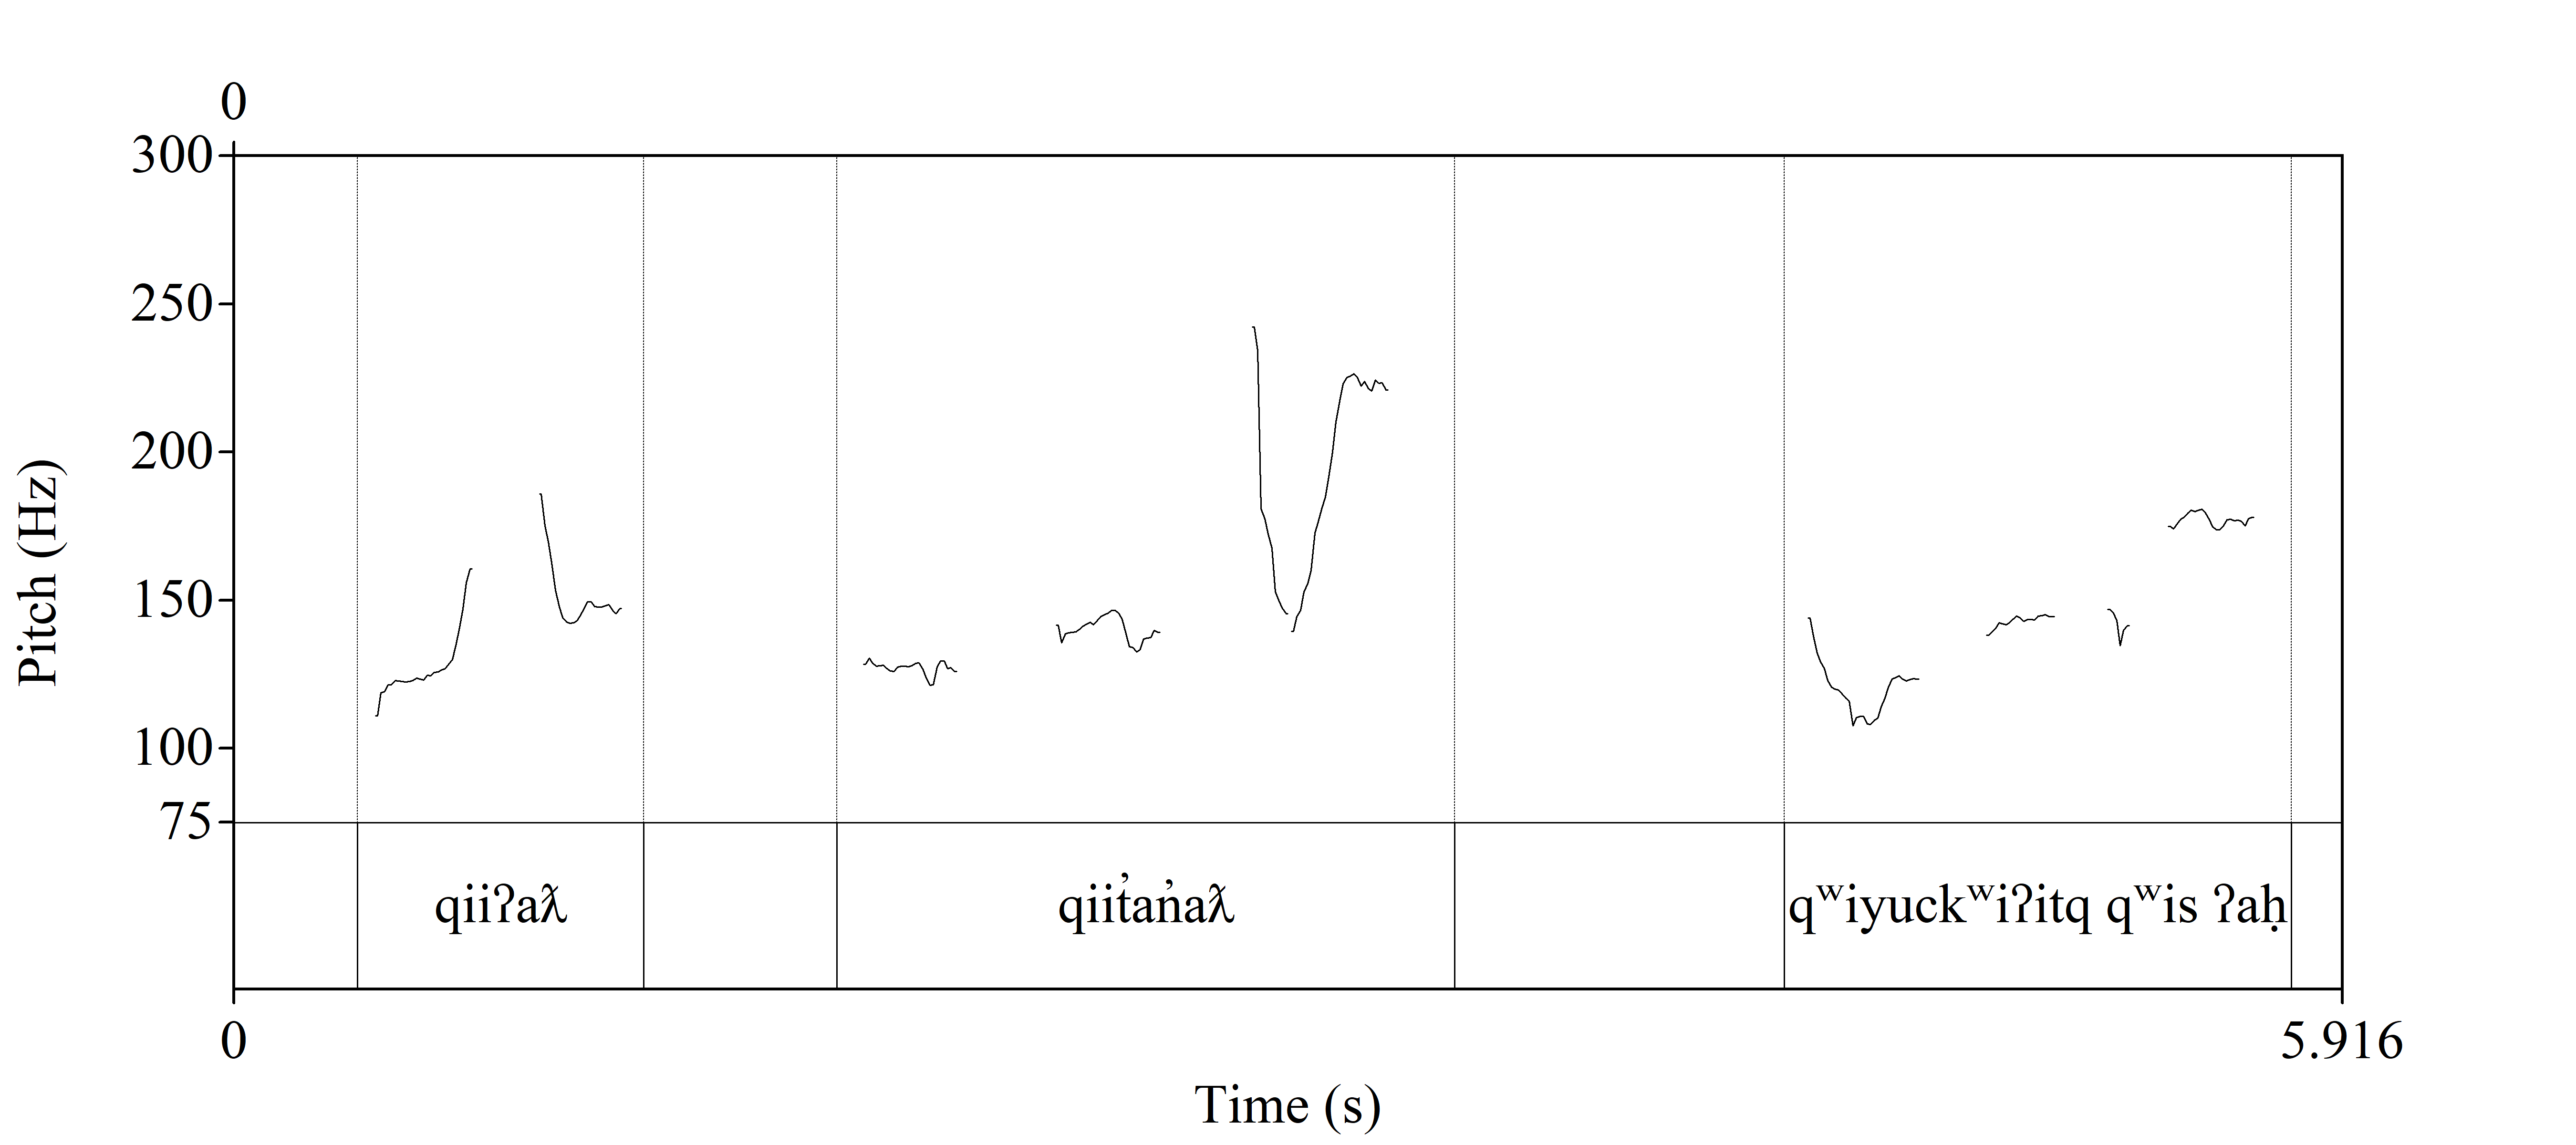
\includegraphics[width=\linewidth]{Kingfisher-001.png}
    \glllll qiiʔaƛ,                  qiit̓an̓aƛ,                         qʷiyuckʷiʔitq        qʷis        ʔaḥ.\\
            qiː‑ʼaƛ                  qiː‑t̓an̓a‑ʼaƛ                      qʷiyu‑ckʷi·‑ʔi·tq    qʷis        ʔaḥ\\
            for.a.long.time‑\gl{fin} for.a.long.time‑slightly‑\gl{fin} time‑done‑\gl{rel.3} happen.thus this\\
            happened.long.ago        quite.a.while.ago                 when.it.occurred     happen.thus this\\
            \gl{pred}                \gl{pred}                         \gl{ref}             \gl{pred}   \gl{ref}\\
            \tln{This happened a long time ago.}
    \exsource[Kingfisher 001]{Louie2003}

    \clearpage

    \ex\label{ex:3.11b}
    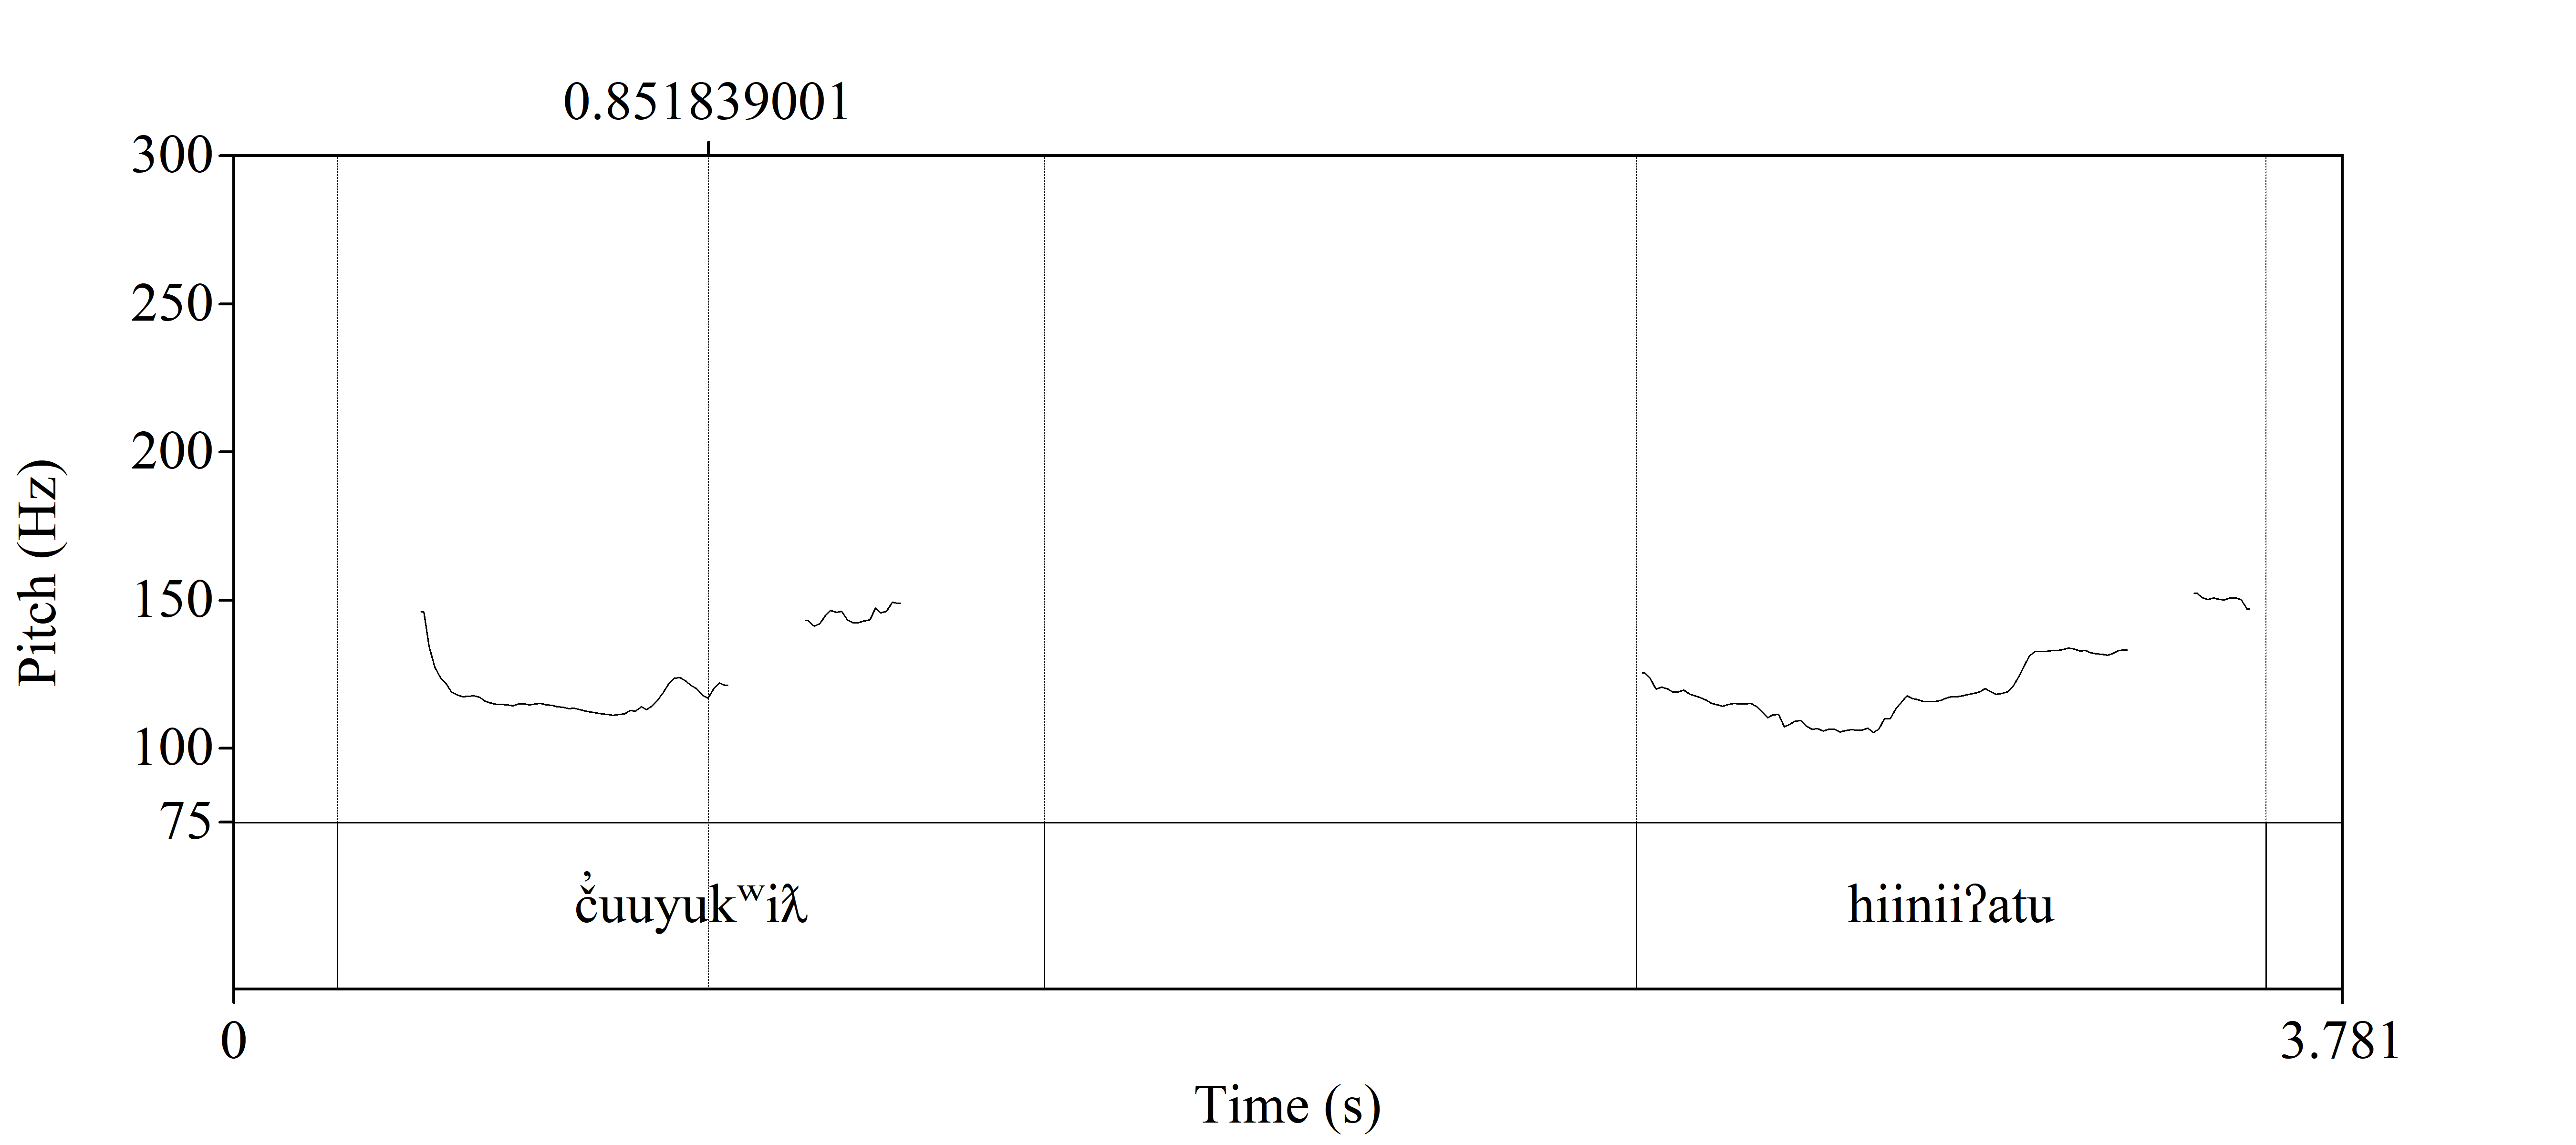
\includegraphics[width=\linewidth]{Qawiqaalth-046.png}
    \glllll č̓uuyukʷiƛ.        hiiniiʔatu.\\
            č̓u‑(y)ukʷi(ƛ)     hin‑ʔi·ʔatu\\
            move‑\gl{incep}   there.\gl{mom}‑get.to.be.under.water\\
            started.migrating dive\\
            \gl{pred}         \gl{pred}\\
            \tln{(The sea lions) started migrating under the water.}
    \exsource[Qawiqaalth 046]{Louie2003}

    \renewcommand{\eachwordfive}{\rmfamily}

  \end{xlist}
\end{exe}

It is important to distinguish these cases of \dfn{clause combining} from \dfn{serialization}. \textcite[98]{Nakayama2001} explains that in cases of serialization, the state of affairs is conceptualized and expressed as a single event, and that in clause combining the state of affairs is conceptualized and expressed as separate events. The same scene can be expressed using either serialization or clause combining, depending on the speaker's choice. Structurally, serialization is distinguished from clause combining by the fact that only the initial predicate will carry person and mood suffixes in cases of serialization. The other members of the serialization immediately follow the main predicate as bare stems. In cases of clause combining, each predicate may take its own mood and participant marking. \textcite[99]{Nakayama2001} provides the following examples showing the contrast between serialization and clause combining respectively.

\clearpage

\begin{exe}
  \ex\label{ex:3.12}
  \exinfo{\idx{Nuuchahnulth} (Wakashan > Southern Wakashan)}
  \begin{xlist}

    \ex\label{ex:3.12a}
    \exinfo{Serialization}
    \glllll mamuukšiƛna               ʔuyi         February\\
            mamuːk‑ši(ƛ)‑na·          ʔuyi         ~\\
            working‑\gl{mom}‑\gl{1pl} at.the.time  February\\
            we.worked                 at.that.time February\\
            \gl{pred}                 \gl{pred}    ~\\
            \tln{We worked in February.}
    \exsource[GL 108]{Louie2003}

    \ex\label{ex:3.12b}
    \exinfo{Clause Combining}
    \glllll ḥayuqʔičḥʔaƛits                    qʷiyaakiis                   qaḥšiƛ        ʔumʔiiqsu.\\
            ḥayu‑qʔičḥ‑ʼaƛ‑it‑s                  qʷiyu‑ʔa·k‑(y)iːs             qaḥ‑ši(ƛ)     ʔumʔi·qsu\\
            ten‑year‑\gl{fin}‑\gl{past}‑\gl{1sg} when‑\gl{poss}‑\gl{indef.1sg} dead‑\gl{mom} mother\\
            I.was.ten.years.old                when.mine.did                died          mother\\
            \gl{pred}                          { }                        \gl{pred}     \gl{ref}\\
            \tln{I was ten years old when my mother died.}
    \exsource[98]{Nakayama2001}

  \end{xlist}
\end{exe}

\noindent Prosody provides additional evidence that speakers conceptualize serialization as a unitary state of affairs, as the pitch traces for \exref{ex:3.13a} and \exref{ex:3.13b} show. The two predicates in \exref{ex:3.13a} fall under the same intonational contour, whereas in \exref{ex:3.13b} they are divided into distinct intonational contours.

\clearpage

\begin{exe}
  \ex\label{ex:3.13}
  \exinfo{\idx{Nuuchahnulth} (Wakashan > Southern Wakashan)}
  \begin{xlist}

    \renewcommand{\eachwordfive}{\rule[-10pt]{0pt}{0pt}\rmfamily}

    \ex\label{ex:3.13a}
    \exinfo{Serialization}\\
    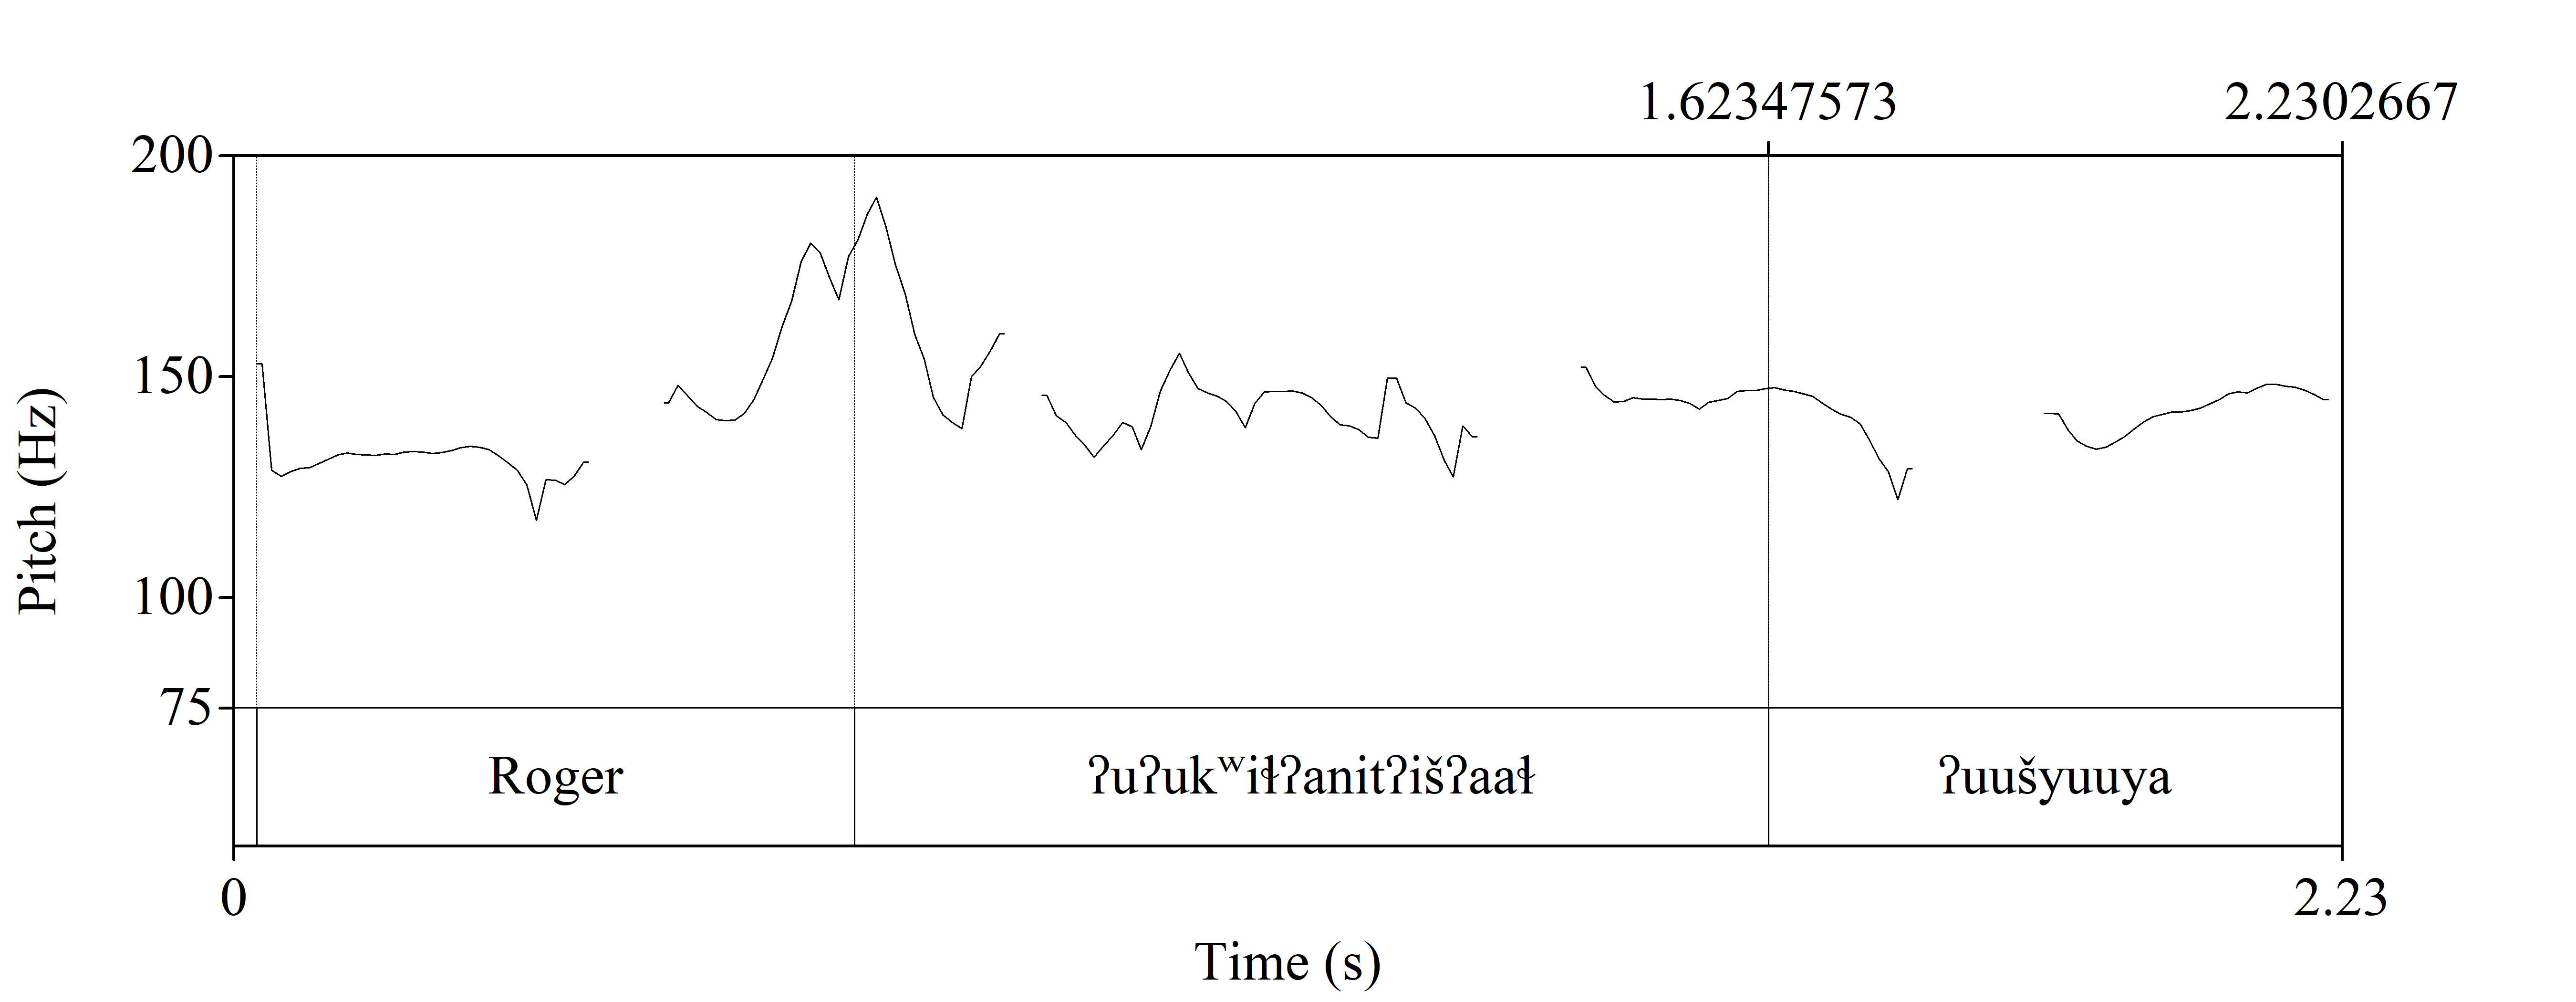
\includegraphics[width=\linewidth]{GL-006.png}
    \glllll Roger     ʔuʔukʷiɬʔanitʔišʔaaɬ                                     ʔuušyuuya,\\
            Roger     \gl{dup}‑ʔu‑kʷiɬ‑ʼat‑it‑ʔi·š‑ʔaːɬ                           ʔuːš‑yuːya\\
            \gl{name} \gl{dup}‑he‑doing.to‑\gl{shift}‑\gl{past}‑\gl{ind.3}‑always some‑at.the.time\\
            Roger     they.used.to.do.it.to.him                                sometimes\\
            \gl{ref}  \gl{pred}                                                \gl{pred}\\
            \tln{sometimes people called him Roger}
    \exsource[GL 006]{Louie2003}

    \ex\label{ex:3.13b}
    \exinfo{Clause Combining}\\
    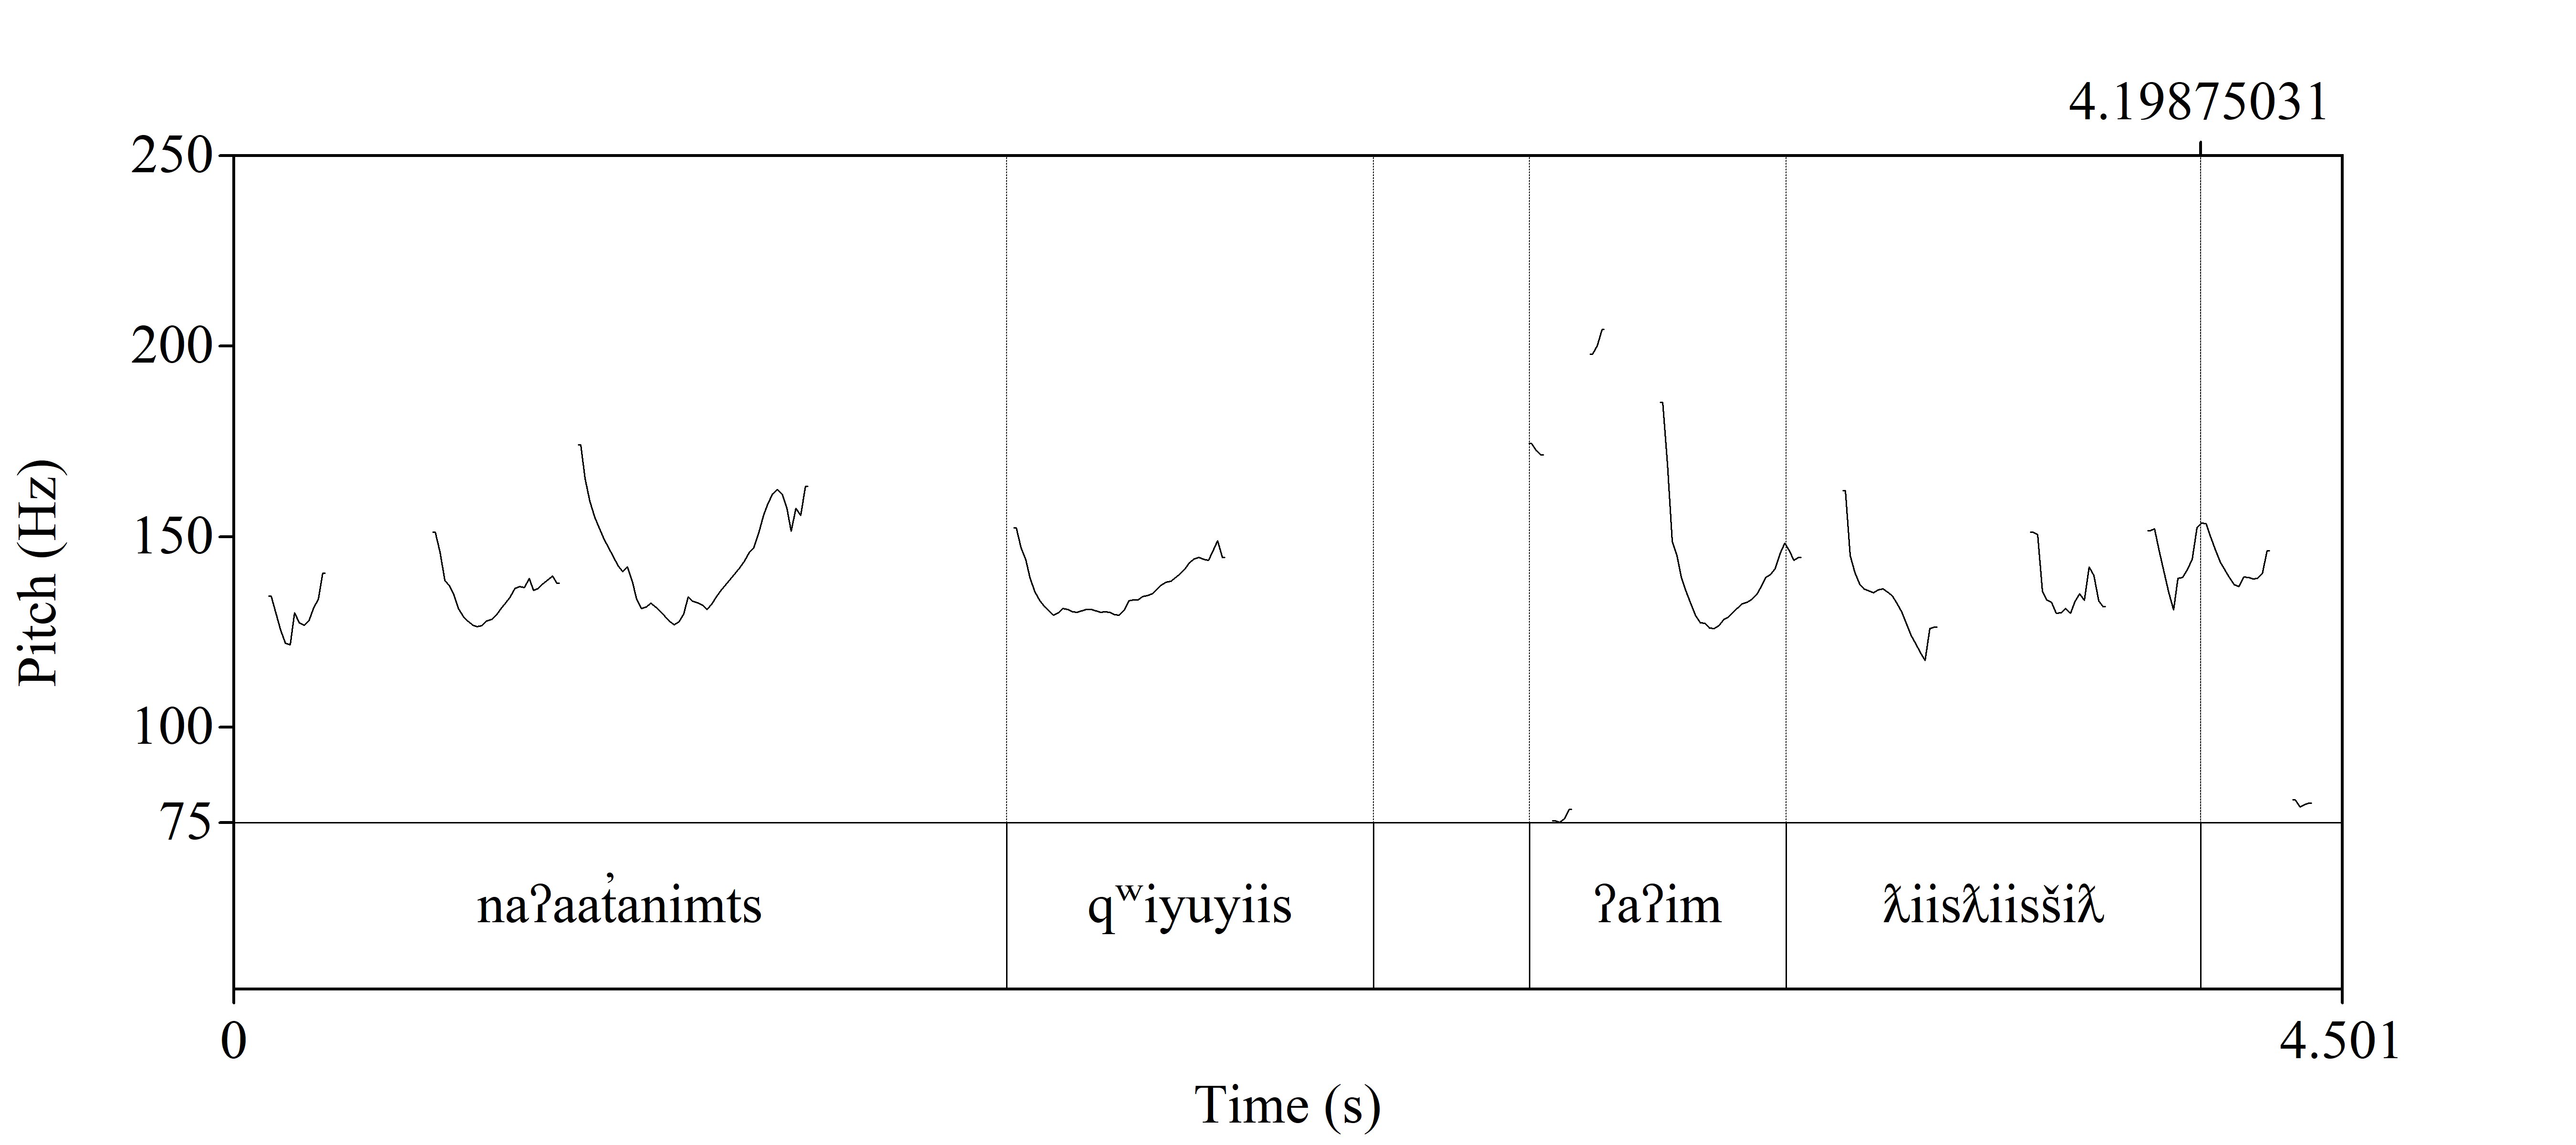
\includegraphics[width=\linewidth]{GL-040.png}
    \glllll naʔaat̓animts                            qʷiyuyiis          ʔaʔim      ƛiisƛiisšiƛ\\
            naʔaːt‑ʼat‑imt‑s                         qʷiyu‑(y)iːs        ʔaʔim      ƛiːsƛiːs‑ši(ƛ)\\
            understand‑\gl{shift}‑\gl{past}‑\gl{1sg} when‑\gl{indef.1sg} first.time go.to.school‑\gl{mom}\\
            I.sort.of.understood                    whenever.I         first.time started.school\\
            \gl{pred}                               { }                \gl{pred} \gl{pred}\\
            \tln{I sort of understood (English) when I first went to school.}
    \exsource[GL 040]{Louie2003}

    \renewcommand{\eachwordfive}{\rmfamily}

  \end{xlist}
\end{exe}

\noindent Additional examples of serialization are below.

\begin{exe}
  \ex\label{ex:3.14}
  \exinfo{\idx{Nuuchahnulth} (Wakashan > Southern Wakashan)}
  \begin{xlist}

    \ex\label{ex:3.14a}
    \glllll  t̓iqʷiɬ           hiiɬ.\\
             t̓iqʷ‑ʽiɬ         hiːɬ\\
             sit‑in.the.house there.in.the.house\\
             sit.on.the.floor there.in.the.house\\
             \gl{pred}        \gl{pred}
             \tln{He was sitting there in the house.}\\
    \exsource[Kingfisher 074]{Louie2003}

    \ex\label{ex:3.14b}
    \glllll wikst̓iiḥʷʼit̓as              kamatquk\\
            wik‑st̓iːḥ‑w̓it̓as             kamatq‑uk\\
            not‑take.direction‑about.to running‑\gl{dur}\\
            without.taking.direction    be.running\\
            \gl{pred}                   \gl{pred}\\
            \tln{He was going to run frantically.}
    \exsource[Mink 135]{Louie2003}

    \ex\label{ex:3.14c}
    \glllll hiikʷaɬšiʔat            k̓ʷačšiʔat.\\
            hiːkʷaɬ‑ši(ƛ)‑ʔa·ɬ      k̓ʷač‑ši(ƛ)‑ʼat\\
            nearly‑\gl{mom}‑\gl{pl} hit.the.right.spot‑\gl{mom}‑\gl{shift}\\
            they.almost.did         hit.the.right.place\\
            \gl{pred}               \gl{pred}\\
            \tln{They almost made a direct hit.}
    \exsource[Wolf 132]{Louie2003}

  \end{xlist}
\end{exe}

For this study, I coded each stem in a serial verb sequence as an individual predicate. In each of the examples in \exref{ex:3.14}, for instance, both words are coded individually as predicates. An alternative approach to the coding of serial verb constructions in Nuuchahnulth would be to consider each sequence of serial verbs as a single complex predicate, and assign just one data point to that complex construction. In this approach, the predicate being analyzed in \exref{ex:3.14a} would not be \txn{t̓iqʷiɬ} \tln{sit on the floor} and \txn{hiiɬ} \tln{there in the house} separately, but instead the single complex predicate \txn{t̓iqʷiɬ hiiɬ} \tln{sit there in the house}. The motivation for this latter approach is the fact, mentioned above, that serial verb constructions are used when the speaker wishes to package the scene as a single state of affairs rather than multiple ones \parencite[98--99]{Nakayama2001}. It may be the case, therefore, that serialized verbs are better treated as a single lexical unit and constitute a single data point rather than multiple ones for the purpose of this study. This would have the presumed effect of significantly reducing the overall polyfunctionality rating for Nuuchahnulth, since there is no structurally unmarked referential counterpart to verb serialization in Nuuchahnulth. That is, a serialized verb construction like \txn{t̓iqʷiɬ hiiɬ} will never be used as a referent without additional structural coding (the relative mood suffix).

However, languages (and individual predicates within a language) vary widely in terms of how lexically unified the components of their serial verb constructions are \parencite[11--12]{Aikhenvald2006}. In some languages, serial verb constructions are highly lexicalized and unified, and one cannot paraphrase them using a sequence of separate clauses and still obtain a felicitous interpretation or the same intended meaning \parencite[6, 11--12]{Aikhenvald2006}. In other languages, serial verb constructions are quite compositional. Nuuchahnulth lies on the compositional end of this spectrum. \textcite[98]{Nakayama2001} notes that Nuuchahnulth speakers may choose to express the same scene either as a single state of affairs (with a serial verb construction) or as multiple states of affairs (with clause combining). Additional evidence of the compositionality of serial verb constructions in Nuuchahnulth is their token frequency: though I have not yet done explicit counts of each combination of verbs in different serial verb constructions, I can confidently assert that individual combinations of verbs in a serial verb construction rarely reoccur beyond their immediate discourse context. Phrases like \txn{t̓iqʷiɬ hiiɬ} \tln{sit there in the house} do not appear to be a lexicalized unit with a conventionally-associated meaning in the same way that English compounds or phrasal verbs are. My decision to code each verb in Nuuchahnulth serial verb constructions as an individual predicate thus reflects the compositionality of those constructions.

Another useful heuristic to keep in mind when determining discourse functions in Nuuchahnulth is that property concepts and numerals/quantifiers are very often predicates, as shown in the following examples. Note that \exref{ex:3.15b} is a serialized predicate construction.

\begin{exe}
  \ex\label{ex:3.15}
  \exinfo{\idx{Nuuchahnulth} (Wakashan > Southern Wakashan)}
  \begin{xlist}

    \ex\label{ex:3.15a}
    \glllll \em{ʔaya}      tukuuk.\\
            \em{ʔaya}      tukuːk\\
            \em{many}      sea.lion\\
            \em{many}      sea.lion\\
            \em{\gl{pred}} \gl{ref}\\
            \tln{There were many kinds of sea lions.}
    \exsource[Qawiqaalth 181]{Louie2003}

    \ex\label{ex:3.15b}
    \glllll \em{ʔaƛac̓asqi}                    \em{ƛ̓iḥuk}       ʕiyaaɬ   t̓uḥc̓iti,\\
            \em{ʔaƛa‑c̓as‑qi·}                  \em{ƛ̓iḥ‑uk}      ʕiyaːɬ   t̓uḥc̓iti\\
            \em{two‑at.the.crown‑on.top}       \em{red‑\gl{dur}} feather  head\\
            \em{two.at.the.crown.of.the.head} \em{red}          feather  head\\
            \em{\gl{pred}}                    \em{\gl{pred}}    \gl{ref} \gl{ref}\\
            \tln{There are two red feathers at the crown of his head.}
    \exsource[Canoe 013]{Louie2003}

    \ex\label{ex:3.15c}
    \glllll \em{p̓išaqʔiš}       ʔiiqḥy̓ak.\\
            \em{p̓išaq‑ʔi·š}     ʔiːqḥ‑y̓ak\\
            \em{bad‑\gl{ind.3}} telling‑instrument\\
            \em{it.is.bad}      news\\
            \gl{pred}           \gl{ref}\\
            \tln{There is bad news.}
    \exsource[Kingfisher 098]{Louie2003}

  \end{xlist}
\end{exe}

\noindent Rarely, however, property words or numerals/quantifiers will be combined into a single intonational contour with the following referent, and in this case they function to modify. Modifiers always precede their referents. One such case is shown in \exref{ex:3.16}.

\begin{exe}
  \ex\label{ex:3.16}
  \exinfo{\idx{Nuuchahnulth} (Wakashan > Southern Wakashan)}\\
  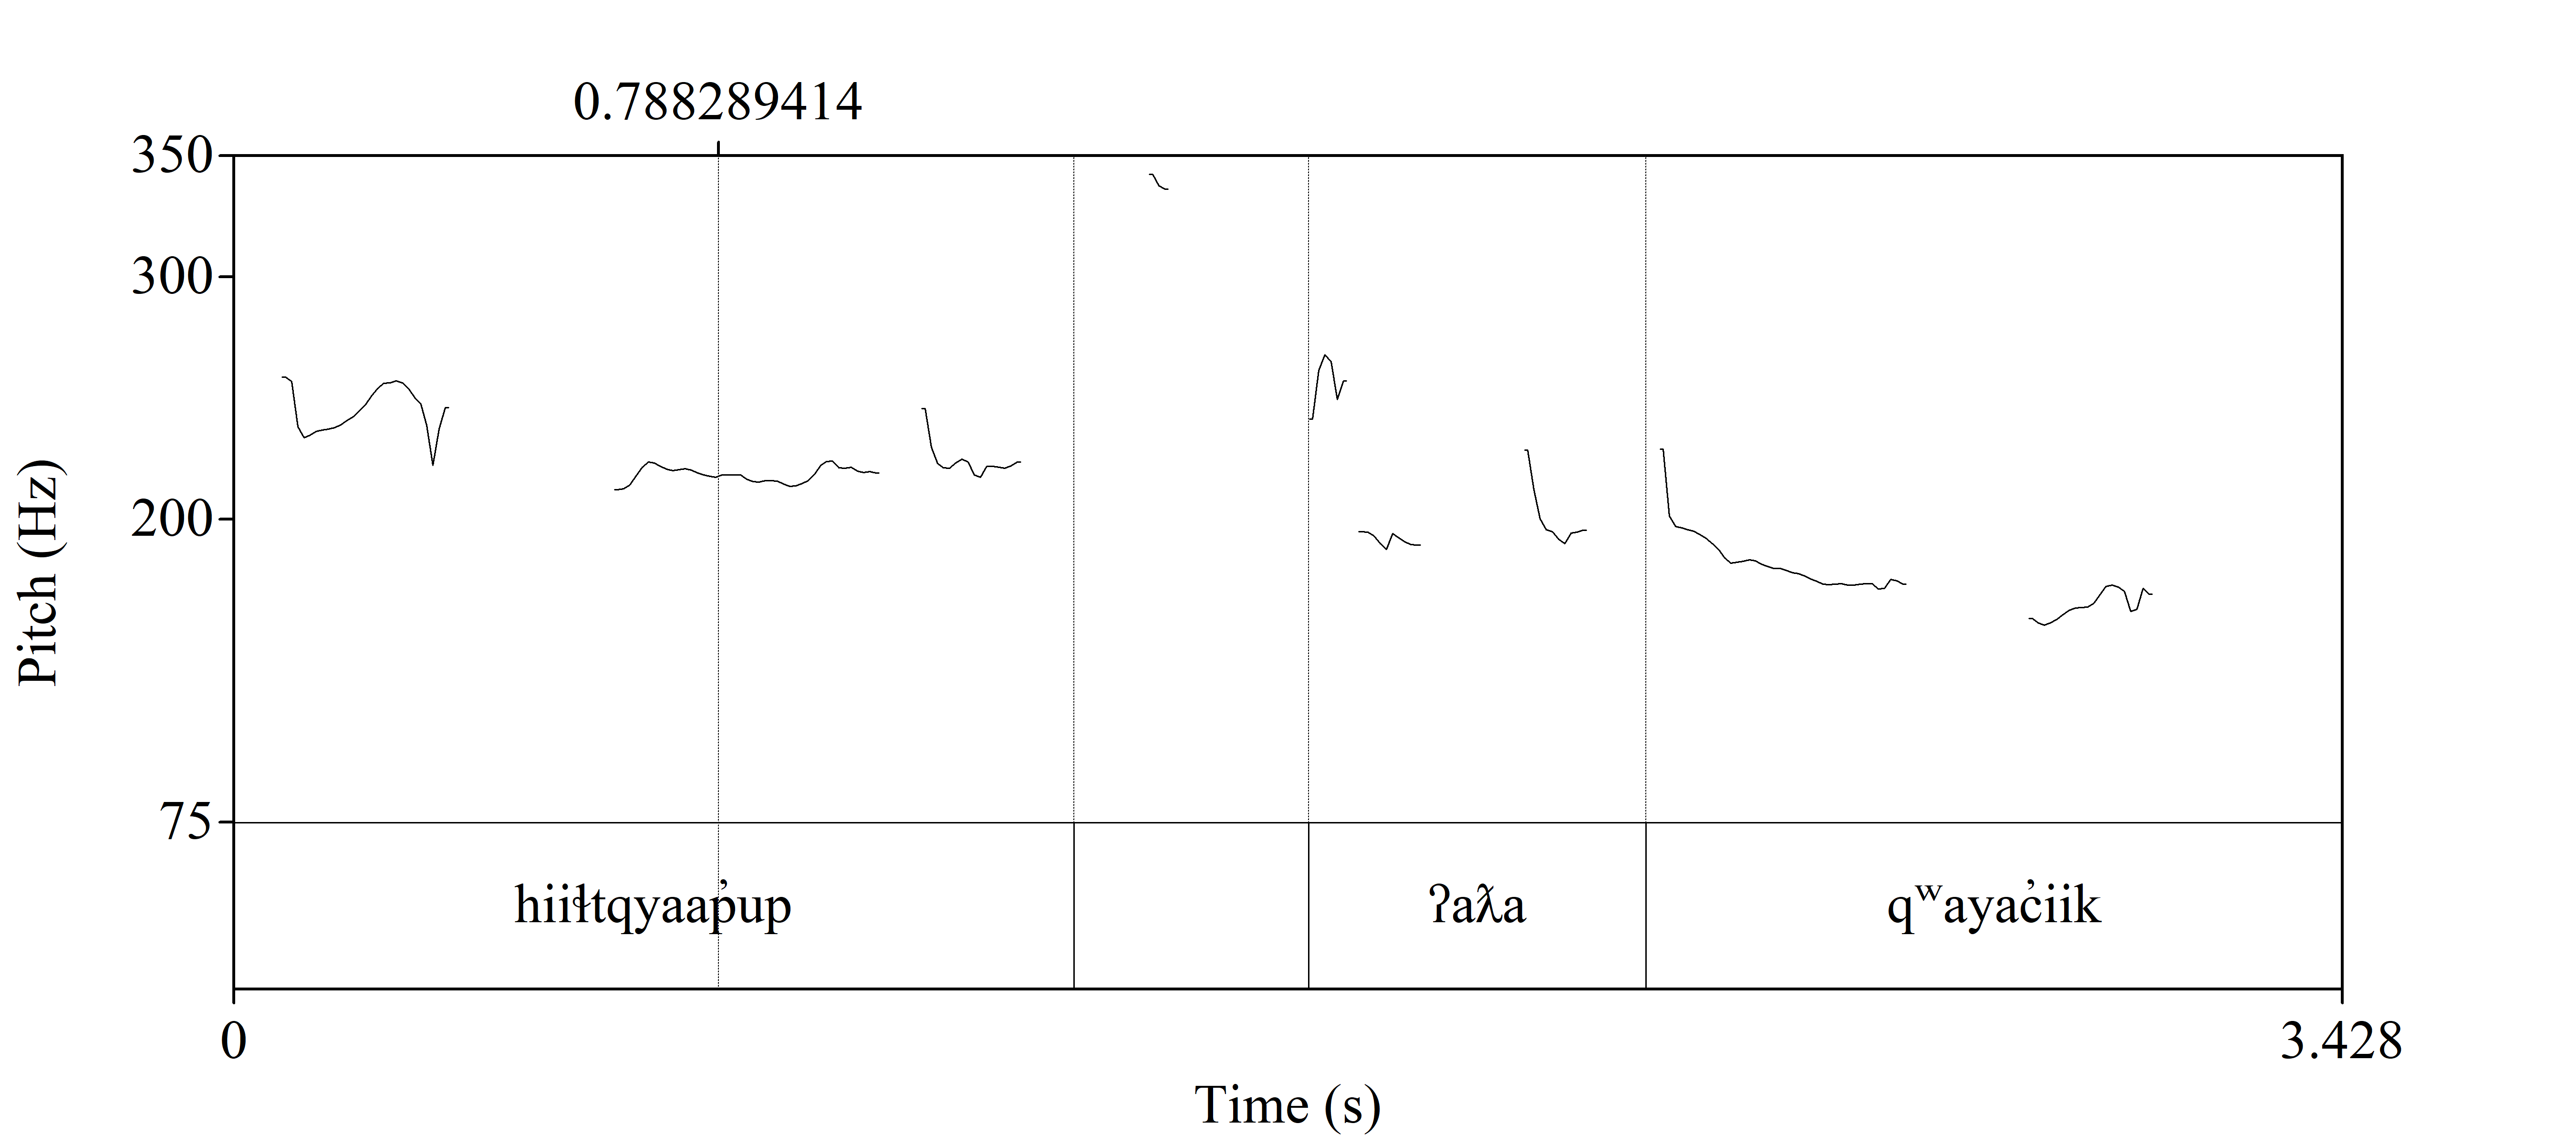
\includegraphics[width=\linewidth]{Wolf-046.png}
  \gllll hiiɬtqyaap̓up            \em{ʔaƛa} qʷayac̓iik.\\
         hiɬ‑tqya·p̓i‑up          \em{ʔaƛa} qʷayac̓iːk\\
         there‑back‑\gl{mom.caus} \em{two}  wolf\\
         put.on.the.back         \em{two}  wolf\\
         \vfix
         \tln{Two wolves put [the dead wolf] on their back.}
  \exsource[FoodThief 046]{Little2003}
\end{exe}

\idx{Nuuchahnulth} does not have any \enquote{adverbial} (predicate modifier) constructions. Meanings that are conveyed by predicate modifiers in other languages are expressed with single predicates or verb serialization in Nuuchahnulth. \citeauthor{Nakayama2001} states, \textquote[{\cite[51]{Nakayama2001}}]{It is, however, difficult to distinguish the structural behavior of such \enquote{adverbs} and that of other intransitive verbals in serialization}. Examples of this kind of serialization are in \exref{ex:3.17}.

\begin{exe}
  \ex\label{ex:3.17}
  \exinfo{\idx{Nuuchahnulth} (Wakashan > Southern Wakashan)}
  \begin{xlist}

    \ex\label{ex:3.17a}
    \glllll sayaʔii       ʔuušyuuya,\\
            saya‑ʔiː      ʔuːš‑yuːya\\
            far.off‑reach some‑at.the.time\\
            went.far      sometimes\\
            \gl{pred}     \gl{pred}\\
            \tln{He went far sometimes.}
    \exsource[Mink 221]{Louie2003}

    \ex\label{ex:3.17b}
    \glllll ʔin      č̓uuy̓iiḥanit                                               ʔaʔum.\\
            ʔin      č̓u‑y̓i·ḥa‑ʼat‑it                                            ʔaʔum\\
            although having.an.odor‑suffering.excessively?‑\gl{shift}‑\gl{past} at.first\\
            although they.smelled.him                                          at.first\\
            { }      \gl{pred}                                                 \gl{pred}\\
            \tln{even though they smelled him at the beginning.}
    \exsource[Qawiqaalth 087]{Louie2003}

    \ex\label{ex:3.17c}
    \glllll ʔaʔums            waɬaak    ʕaʔuknak  1919\\
            ʔaʔum‑s           waɬaːk    ʕaʔuknak  { }\\
            at.first‑\gl{1sg} go        \gl{name} { }\\
            I.first           went      Auknak    { }\\
            \gl{pred}         \gl{pred} \gl{ref}  { }\\
            \tln{I first went to Auknak in 1919.}
    \exsource[GL 029]{Louie2003}

    \ex\label{ex:3.17d}
    \glllll qiičiʔaƛs                          suutiɬ       ḥaaḥuupa\\
            qiː‑či(ƛ)‑ʼaƛ‑s                     sut‑(č)iɬ    ḥaːḥuːp‑(y)a·\\
            for.long‑\gl{mom}‑\gl{fin}‑\gl{1sg} you‑doing.to teaching‑\gl{cont}\\
            I.have.been.doing.for.long         to.you       teaching\\
            \gl{pred}                          \gl{pred}    \gl{pred}\\
            \tln{I have been teaching you (how to fish) for a long time.}
    \exsource[GL 115]{Louie2003}

  \end{xlist}
\end{exe}

Certain inflectional markers, when present, also unambiguously indicate the discourse function of the word they appear with. Words which take the Definite suffix \txn{-ʔi·} (glossed as \gl{def}) or one of the Relative suffixes (glossed as \gl{rel}) always function to refer.

The status of the Definite marker in Nuuchahnulth and its parallels / cognates in other Pacific Northwest languages is a matter of some debate. Here, I treat it as an inflectional marker which incidentally and unambiguously indicates that the word it attaches to is a referent. While \textcite[48]{Nakayama2001} does explicitly talk about \enquote{nominalization with the use of \txn{‑ʔi·} \textsc{definite}}, he does not explicitly call the suffix a nominalizer or label it as such. And while the examples in \textcite[48]{Nakayama2001} do indeed make the Definite suffix appear derivational in nature, these examples are not representative. The majority of uses of the Definite suffix in the Nuuchahnulth corpus occur with typical object words rather than action words. In one text (Bluejay), 10 out of 13 instances of the Definite suffix occur with object words. Given this distribution, it seems more accurate to state that the Definite suffix is inflectional, and incidentally happens to indicate that the word is a referent, than that it is derivational.

Other inflectional markers also unambiguously indicate the discourse function of the word they appear with. Except when they co-occur with either the Definite or Relative markers, the following kinds of mood suffixes always indicate a predicate. In \idx{Nuuchahnulth}, most mood suffixes are fused with the following person suffixes, so each of the suffixes in this list has multiple realizations depending on the person and number of the clausal arguments.

\begin{itemize}
  \singlespacing
  \item conditional (\gl{cond})
  \item dubitive (\gl{dub})
  \item imperative (\gl{imp})
  \item indicative (\gl{ind})
  \item interrogative (\gl{inter})
  \item purposive (\gl{purp})
  \item quotative (\gl{quot})
  \item subordinate (\gl{subord})
\end{itemize}

\noindent In serial verb constructions (discussed above), these mood suffixes only appear on the first (main) stem in a serial verb construction \parencite[42]{Nakayama2001}. Main predicates are also predominantly marked for person even if mood marking is not present (over 90\% of main predicates in the first person) \parencite[29]{Nakayama2001}. Aspect markers, however, are not a completely reliable indicator of predication. Though it happens infrequently, aspect markers may occur with referents or modifiers as well \parencite[47--50]{Nakayama2001}.

Certain distributional behaviors also abet identification of the discourse function of a word. \citeauthor{Nakayama2001} notes the following in regard to referents: \textquote[{\cite[49]{Nakayama2001}}]{Nominals can be modified with expressions of property concepts, quantity, or quantifiers, but not directly with qualifying expressions like \txn{hiikʷaɬ} \tln{almost} or \txn{ʔanatʼuu} \tln{barely}.}. Syntactic patterns are also helpful: Negation is accomplished by means of a negative predicate \txn{wik-}, which takes another predicate as its complement. Modifiers generally precede their heads, whether the head is a referent or predicate. As mentioned above, in serial verb constructions, only the main predicate takes person and mood marking, and the other members of the serialization immediately follow the main predicate as bare stems.\index{Nuuchahnulth}

Finally, discourse-level considerations play an important role in determining the pragmatic function of each word. Most helpful is topic continuity, wherein a referent is already established in the discourse. This is accomplished either directly via an overt referent in a lexical argument or bound person marker, or indirectly via other kinds of inflectional affixes or features of a word that imply the existence of a referent \parentext{what \textcite{Kibrik2011} calls \dfn{referential aids}}. Each successive lexical item encountered in a text must be interpreted in the context of the previously established discourse referents, so that certain interpretations of the item are much more sensible than others. Lastly, I consulted the audio files accompanying the corpus in order to take prosodic information into account. Clear prosodic breaks in the discourse are a strong sign of clausal boundaries.\index{Nuuchahnulth}

What follows is a sample annotated abstract from the beginning of the Kingfisher story \parencite{Louie2003}, with each relevant lexical item annotated for its discourse function. Lexical items that are excluded from this study for one of the reasons discussed in \secref*{sec:3.3.1} are not given an annotation. Following this passage, the reasons for each coding decision are provided in bullet point format. Each point may apply to multiple lexical items, and vice versa. The tokens that each point applies to are indicated at the beginning of that bullet point.

\clearpage

\begin{exe}

  \ex\label{ex:3.18}
  \exinfo{\idx{Nuuchahnulth} (Wakashan > Southern Wakashan)}
  \singlespacing
  \renewcommand{\eachwordfive}{\rule[-10pt]{0pt}{0pt}\rmfamily}

  \glllll qiiʔaƛ\super{1}          qiit̓an̓aƛ\super{2}                 qʷiyuckʷiʔitq\super{3} qʷis\super{4} ʔaḥ\super{5}\\
          qiː‑ʼaƛ                  qiː‑t̓an̓a‑ʼaƛ                      qʷiyu‑ckʷi·‑ʔi·tq      qʷis          ʔaḥ\\
          for.a.long.time‑\gl{fin} for.a.long.time‑slightly‑\gl{fin} time‑done‑\gl{rel.3}   happen.thus   this\\
          happened.long.ago        quite.a.while.ago                 when.it.occurred       happen.thus   this\\
          \gl{pred}                \gl{pred}                         { }                    \gl{pred}     \gl{ref}\\
          \vfix
          \tln{This happened a long time ago.}

  \glllll siikc̓inƛ\super{6}  siikaa\super{7}   hitac̓inƛ\super{8}         maaqtusiis\super{9}\\
          siːk‑c̓inƛ          siːk‑(y)a·        hita‑c̓inƛ                 maːqtusiːs\\
          sailing‑into.a.bay sailing‑\gl{cont} there.\gl{mom}‑into.a.bay \gl{name}\\
          sail.into.a.bay    sailing           entered.into.a.bay        \gl{name}\\
          \gl{pred}          \gl{pred}         \gl{pred}                 \gl{ref}\\
          \vfix
          \tln{They sailed into the bay of Maaqtusiis.}

  \glllll yuupickʷimatak\super{10}    yuupi\super{11} yuksaaʔa\super{12}\\
          yuːpi‑ckʷi·‑matak           yuːpi           yu‑ksa·ʔa\\
          breeze‑done‑probably        breeze          blowing‑come.to.land\\
          probably.there.was.a.breeze breeze          breeze.along.the.shoreline\\
          \gl{pred}                   \gl{ref}        \gl{pred}\\
          \vfix
          \tln{There probably was a little wind, blowing towards the land.}

  \glllll qʷiyimtii\super{13}         n̓aas\super{14} hitac̓inƛ\super{15}\\
          qʷiyu‑imt‑(y)iː             n̓aːs           hita‑c̓inƛ\\
          when‑\gl{past}‑\gl{indef.3} day            there.\gl{mom}‑in.a.bay\\
          whenever.it.was             day            entered.a.bay\\
          { }                         \gl{ref}       \gl{pred}\\
          \vfix
          \tln{They came into the bay one day.}

  \glllll hitac̓u\super{16} ʔukɬaakʔakna\super{17}                y̓uuqʷaa\super{18}\\
          hitac̓u           ʔu‑kɬa·‑ak‑ʔa·k‑na·                   y̓uːqʷaː\\
          \gl{name}        it‑called‑\gl{dur}‑\gl{poss}‑\gl{1pl} also\\
          \gl{name}        we.also.call.it                       also\\
          { }              \gl{pred}                             \gl{pred}\\
          \vfix
          \tln{We also call it (the bay) ``\txn{hitac̓u}".}

  \glllll waɬyuu\super{19} maaqtusiis\super{20} wiiḥaaqsusiis\super{21}\\
          waɬ‑yu·          maːqtusiːs           wiːḥaːqsusiːs\\
          go.home‑done     \gl{name}            \gl{name}\\
          gone.home        \gl{name}            \gl{name}\\
          \gl{pred}        \gl{ref}             { }\\
          \vfix
          \tln{They went to Maaqtusiis — [to be exact,] \txn{Wiiḥaaqsusiis}.}

  \glllll ʔuʔiiyačištckʷi\super{22} wiiḥaaqsusiis\super{23} t̓ayuukʷiƛ\super{24} kuunaa\super{25}\\
          ʔu‑ʔi·ya‑ačišt‑ckʷi·      wiːḥaːqsusiːs           t̓ayuː‑kʷi(ƛ)        kuːnaː\\
          it‑reach‑on.the.sea‑done  \gl{name}               anchored‑\gl{mom}   schooner\\
          reached                   \gl{name}               anchored            schooner\\
          \gl{pred}                 \gl{ref}                \gl{pred}           \gl{ref}\\
          \vfix
          \tln{The schooner reached \txn{Wiiḥaaqsusiis} and dropped anchor.}

  \glllll wik\super{26} ʔiiḥ\super{27} wikckʷii\super{28} ʔiiḥ\super{29}\\
          wik           ʔiːḥ           wik‑ckʷi·          ʔiːḥ\\
          not           large          not‑done           large\\
          not           large          was.not            large\\
          \gl{pred}     \gl{pred}      \gl{pred}          \gl{pred}\\
          \vfix
          \tln{It (the schooner) was not so big.}

  \glllll ʔaƛa\super{30} ʔaƛista\super{31}   qacc̓istamitquu\super{32}\\
          ʔaƛa           ʔaƛa‑ista           qacc̓a‑ista‑mit‑quː\\
          two            two‑people.on.board three‑people.on.board‑\gl{past}‑\gl{cond.3}\\
          two            two.people.on.board there.could.have.been.three.people.on.board\\
          \gl{pred}      \gl{ref}            \gl{pred}\\
          \vfix
          \tln{There were two crewmen, or there could have been three, on the ship.}

  \glllll hinaačiƛ̓aɬ\super{33}                  yaqitii\super{34}\\
          hin‑a·či(ƛ)‑ʔa·ɬ                      yaq‑it‑(y)iː\\
          there.\gl{mom}‑go.out.to.meet‑\gl{pl} who‑\gl{past}‑\gl{indef.3}\\
          they.go.out.to.meet                   whoever.it.was\\
          \gl{pred}                             { }\\
          \vfix
          \tln{Some people went out to meet them (the people on the schooner).}

  \clearpage

  \glllll ʔin\super{35} ʔutwiickʷiʔaaɬ\super{36} hinaačiƛ\super{37}            wiʔakʔi\super{38} wiiʔaksaʔi\super{39} ḥaaʔak̓atʔi\super{40}      ɬim̓aqsti\super{41}\\
          ʔin           ʔutwiː‑ckʷi·‑ʔaːɬ        hin‑a·či(ƛ)                   wiʔak‑ʔi·         wiʔak‑sa‑ʔi·         ḥaːʔak‑ʼat‑ʔi·            ɬim̓aqsti\\
          since         first‑done‑always        there.\gl{mom}‑go.out.to.meet brave‑\gl{def}    brave‑real‑\gl{def}  strong‑\gl{poss}‑\gl{def} mind\\
          since         they.were.the.first.one  go.out.to.meet                the.brave.one     the.bravest.one      the.one.with.strong.one   mind\\
          { }           \gl{pred}                \gl{pred}                     \gl{ref}          \gl{ref}             \gl{ref}                  \gl{ref}\\
          \vfix
          \tln{The first ones to go out were the bravest ones, the ones with strong minds.}

  \glllll ʔin\super{42} naʔaackʷaƛ\super{43} ʔaya\super{44} mamaɬn̓i\super{45} hisiickʷiʔitqʔaɬ\super{46} hiistiƛ\super{47} ciqy̓ak\super{48} čiinuukʔatḥ\super{49}\\
          ʔin           naʔaː‑ckʷi·‑ʼaƛ      ʔaya           mamaɬn̓i           hisiː‑ckʷi·‑ʔi·tq‑ʔa·ɬ     hiːstiƛ           ciq‑y̓akʷ         č̓iːnuːk‑ʼatḥ\\
          ??            hear‑done‑\gl{fin}   many           white.man         ??‑done‑\gl{rel.3}‑\gl{pl} from              speak‑instrument Chinook‑belonging.to\\
          ??            understood           many           white.man         the.way.they.spoke         from              language         Chinook\\
          { }           \gl{pred}            \gl{mod}       \gl{ref}          { }                        \gl{pred}         \gl{ref}         \gl{ref}\\
          \vfix
          \tln{Many white men could understand Chinook Jargon.}

  \glllll čiičiinukʷackʷaƛ\super{50}                      ʔuuš\super{51}\\
          \gl{dup}‑čiːnu·k‑(y)a‑ckʷi·‑ʼaƛ                 ʔuːš\\
          \gl{distr}‑speak.Chinook‑\gl{rep}‑done‑\gl{fin} some\\
          spoke.Chinook.Jargon                            some\\
          \gl{pred}                                       \gl{ref}\\
          \vfix
          \tln{Some of them spoke Chinook Jargon.}

  \glllll hist̓atḥckʷaƛukʔaɬ\super{52}                        ʔaḥ\super{53} [Hudson Bay]\\
          hist‑ʼatḥ‑ckʷi·‑ʼaƛ‑uk‑ʔa·ɬ                        ʔaḥ           ~\\
          there‑belonging.to‑done‑\gl{fin}‑\gl{poss}‑\gl{pl} this          ~\\
          they.got.theirs.from.there                         they          ~\\
          \gl{pred}                                          \gl{ref}      { }\\
          \vfix
          \tln{They got theirs (= their knowledge of Chinook Jargon) from Hudson Bay Company.}

  \glllll yaqʷiiyii\super{54}     naʔaaʔaƛ\super{55} Captainmitquu\super{56}       yaqʷacʔitq\super{57}        šipʔii\super{58}\\
          yaqʷ‑wi·‑(y)iː          naʔaː‑ʼaƛ          Captain‑mit‑quː               yaqʷ‑ac‑ʔi·tq               šip‑ʔi·\\
          who‑first‑\gl{indef.3}  hear‑\gl{fin}      captain‑\gl{past}‑\gl{cond.3} who‑belonging.to‑\gl{rel.3} ship‑\gl{def}\\
          the.ones.who.were.first understood         one.who.was.Captain           owner.of                    the.ship\\
          { }                     \gl{pred}          \gl{pred}                     { }                         \gl{ref}\\
          \vfix
          \tln{Among the first ones that [learned to] understand the language might have been the Captain who was taking command of the ship.}

  \parencite[Kingfisher]{Louie2003}
  \renewcommand{\eachwordfive}{\rmfamily}

\end{exe}

\begin{itemize}
  \singlespacing
  \item {[\txn{qiiʔaƛ}\super{1}; \txn{qʷis}\super{4}; \txn{siikc̓inƛ}\super{6}; \txn{siikaa}\super{7}; \txn{yuupickʷimatak}\super{10}; \txn{yuksaaʔa}\super{12}; \txn{hitac̓inƛ}\super{15}; \txn{waɬyuu}\super{19}; \txn{ʔuʔiiyačištckʷi}\super{22}; \txn{t̓ayuukʷiƛ}\super{24}; \txn{wik}\super{26}; \txn{wikckʷii}\super{28}; \txn{ʔaƛa}\super{30}; \txn{qacc̓istamitquu}\super{32}; \txn{hinaačiƛ̓aɬ}\super{33}; \txn{ʔutwiickʷiʔaaɬ}\super{36}; \txn{naʔaackʷaƛ}\super{43}; \txn{hiistiƛ}\super{47}; \txn{čiičiinukʷackʷaƛ}\super{50}; \txn{hist̓atḥckʷaƛukʔaɬ}\super{52}; \txn{Captainmitquu}\super{56}]} \textsc{pred:} These words are in initial position in their clause, with no obvious topicalization or focus construction which would trigger another item to precede them.
  \item {[\txn{qiit̓an̓aƛ}\super{2}; \txn{hitac̓inƛ}\super{8}; \txn{y̓uuqʷaa}\super{18}; \txn{ʔiiḥ}\super{27}; \txn{ʔiiḥ}\super{29}; \txn{hinaačiƛ}\super{37}; \txn{naʔaaʔaƛ}\super{55}]} \textsc{pred:} These words are serialized predicates, immediately following another predicate, with no person or mood marking (i.e. as a bare stem), and can be reasonably interpreted as one part of a single state of affairs rather than separate states of affairs.
  \item {[\txn{ʔaḥ}\super{5}; \txn{maaqtusiis}\super{9}; \txn{yuupi}\super{11}; \txn{n̓aas}\super{14}; \txn{maaqtusiis}\super{20}; \txn{wiiḥaaqsusiis}\super{23}; \txn{kuunaa}\super{25}; \txn{ʔaƛista}\super{31}; \txn{wiʔakʔi}\super{38}; \txn{mamaɬn̓i}\super{45}; \txn{ciqy̓ak}\super{48}; \txn{ʔuuš}\super{51}; \txn{ʔaḥ}\super{53}; \txn{šipʔii}\super{58}]} \textsc{ref:} These words fill either the Subject or Object slot immediately following the predicate or serialized predicate construction. Subjects and Objects rarely co-occur in Nuuchahnulth clauses, making the post-predicate position a useful heuristic for reference.
  \item {[\txn{yuksaaʔa}\super{12}]} \textsc{pred:} These words constitute their own prosodic unit, and thus likely are functioning as the predicative head of their clause. In particular, these words come at the end of the larger utterance, and seem to be antitopics.
  \item {[\txn{ʔukɬaakʔakna}\super{17}; \txn{qacc̓istamitquu}\super{32}; \txn{hinaačiƛ̓aɬ}\super{33}; \txn{hist̓atḥckʷaƛukʔaɬ}\super{52}; \txn{Captainmitquu}\super{56}]} \textsc{pred:} These words take person and/or mood inflection.
  \item {[\txn{wiʔakʔi}\super{38}; \txn{wiiʔaksaʔi}\super{39}; \txn{ḥaaʔak̓atʔi}\super{40}; \txn{šipʔii}\super{58}]} \textsc{ref:} These words take the Definite suffix \txn{-ʔi·}.
  \item {[\txn{ʔaya}\super{44}]} \textsc{mod:} This word enriches the meaning of the following referent, and fills the modifier slot immediately preceding it. It also forms part of the same prosodic unit as the following referent.
\end{itemize}

Words that are not coded for their discourse function are either a) proper names, b) uninterpretable by \textcite{Nakayama2001}, or c) contain overt derivation (the Relative or Indefinite suffixes).

One final note on the negative predicate \txn{wik‑}: \textcite[119--122]{Nakayama2001} treats this stem like any other lexical predicate. While in many languages negation is primarily a grammatical phenomenon (i.e. it is coded through grammatical affixes or otherwise highly-grammaticalized words), in Nuuchahnulth negation appears to be primarily a lexical phenomenon accomplished with complement-taking predicates such as \txn{wik‑} \tln{not} and \txn{wiiy̓a} \tln{never}. This distinction between lexical and grammatical negation is analagous to the distinction between lexical and grammatical aspect. Behaviorally, negative constructions in Nuuchahnulth act just like other lexical complement-taking predicates, including allowing for the presence of lexical suffixes, e.g. \txn{wik‑maɬ} \tln{not-surviving}. Because these negators are more lexical than grammatical for Nuuchahnulth, they are treated as lexical items and given an analysis in this study (usually but not always as predicates).

The complete set of annotations for the Nuuchahnulth corpus may be found at \href{https://github.com/dwhieb/dissertation}{https://github.com/\\dwhieb/dissertation}.

\section{Analysis}
\label{sec:3.4}

This section discusses the specific statistical measures used in this study. In \secref*{sec:3.4.1}, I present the measure used to quantify the lexical polyfunctionality of individual items in a corpus, and in \secref*{sec:3.4.3} I discuss the use of token frequencies versus dispersion.

\subsection{Measuring lexical polyfunctionality}
\label{sec:3.4.1}

Once the lexical tokens in a corpus are annotated for their discourse functions, it is possible to calculate the functional diversity of each lexical item using a measure known as Shannon's diversity index. This section summarizes the rationale for using this metric and the procedure for calculating it.

Intuitively speaking, a lexical item is most functionally diverse when it is used with equal frequency for reference, predication, and modification. A perfectly polyfunctional lexical item which appears 300 times a corpus would therefore have a distribution like that in \tabref{tab:perfectly-polyfunctional}. By contrast, a perfectly monofunctional lexical item with the same overall frequency would have a distribution like that in \tabref{tab:perfectly-monofunctional}. What is needed is a metric that captures how evenly distributed the tokens of a lexical item are across the different discourse functions. A perfectly polyfunctional item like that in \tabref{tab:perfectly-polyfunctional} should receive a high rating (say, $1$), while a perfectly monofunctional item like that in \tabref{tab:perfectly-monofunctional} should receive a low rating (say, $0$).

\begin{table}[h]
  \centering
  \caption{Distribution of discourse functions for a perfectly polyfunctional lexical item}
  \label{tab:perfectly-polyfunctional}
  \begin{tabular}{ l c c c }
    \toprule
    lexical item & reference & predication & modification\\
    \midrule
    \txn{stem}   & 100       & 100         & 100\\
    \bottomrule
  \end{tabular}
\end{table}

\begin{table}[h]
  \centering
  \caption{Distribution of discourse functions for a perfectly monofunctional lexical item}
  \label{tab:perfectly-monofunctional}
  \begin{tabular}{ l c c c }
    \toprule
    lexical item & reference & predication & modification\\
    \midrule
    \txn{stem}   & 300       & 0           & 0\\
    \bottomrule
  \end{tabular}
\end{table}

I elected to use Shannon's diversity index ($H$) for this purpose \parencites{Shannon1948}{Shannon1951}. Originally devised as a measure of entropy in text (uncertainty or information content), the Shannon index has also become a popular measure of species diversity in ecology \parencites{Avolioetal2012} and attention diversity in political science \parencite{BoydstunBevanThomas2014}. Here I am using it as a measure of the functional diversity of lexical items. The normalized version of Shannon's $H$ yields a value between $0$ (low diversity) and $1$ (high diversity). For a categorical variable with $n$ possible values, $H_{norm}$ is calculated using the formula in \exref{ex:Shannon-H}, where $p_i$ corresponds to the percent frequency of the $i$\textsuperscript{th} possible value of the variable.

\begin{exe}
  \ex\label{ex:Shannon-H}
  $H_{norm} = \displaystyle\frac{-\displaystyle\sum_{i = 1}^{n}(p_i \cdot \ln p_i)}{\ln n}$
\end{exe}

\noindent For this study, $n$ will always be $3$ (reference, predication, and modification). Future researchers may wish to adjust this number depending on the number of discourse functions examined (for example, if the predicate modifier function were included).

Frequently there will not be any instances of a lexical item being used in one discourse function or another. Since $\log 0$ is undefined, the above formula cannot be resolved in these cases. One common workaround to this problem is to increment the frequencies of each discourse function by $1$ before performing the calculation. Another is to simply treat $\log 0$ as equal to $0$ \parencite[120--121]{Gries2013}. I use the latter procedure in this study.

Applying Shannon's $H$ to the fabricated data in \tabref{tab:perfectly-polyfunctional} and \tabref{tab:perfectly-monofunctional} produces the desired results: a value of $1$ for $H$ in the perfectly polyfunctional case and a value of $0$ in the perfectly monofunctional case.

One limitation of the Shannon diversity index as applied to this study stems from the fact that there are so few discourse functions under consideration (just three: reference, predication, and modification). This means that at low frequencies there are a limited number of possible values of Shannon's $H$. For example, a lexical item with a frequency of $2$ will either have an $H$ value of $0$ or $.63$, because there are only two ways those tokens can be distributed across discourse functions ($2\ 0\ 0$ or $1\ 1\ 0$). A lexical item with a frequency of $3$ will have an $H$ value of $0$, $.58$, or $1$, because there are only three ways those tokens can be distributed across discourse functions ($3\ 0\ 0$, $2\ 1\ 0$, or $1\ 1\ 1$), and so on.

To address this issue, I only included lexical items in the samples that had a raw frequency of at least $4$. This cutoff was established based on the fact that $4$ is the smallest frequency that can theoretically return a significant result for Shannon's $H$ when a lexical item is maximally functionally diverse, in one of the two ways one can compute a multinomial test (probabilities vs. a χ\textsuperscript{2} test).

Another consideration when determining how to calculate lexical polyfunctionality is whether the counts of each function type (reference, predication, and modification) should first be normalized to their overall incidence in the corpus before being used for the calculation of Shannon's $H$. For example, Nuuchahnulth displays a relatively low overall incidence of modification, as \tabref{tab:Nuuchahnulth-function-proportions} shows.

\begin{table}[h]
  \centering
  \caption{Distribution of discourse functions in Nuuchahnulth}
  \label{tab:Nuuchahnulth-function-proportions}
  \begin{tabular}{ l r r }
    \toprule
    discourse function & token frequency & percentage\\
    \midrule
    modification &    81 &   1.07\%\\
    predication  & 5,049 &  67.17\%\\
    reference    & 2,387 &  31.75\%\\
    \midrule
    total        & 7,517 & 100.00\%\\
    \bottomrule
  \end{tabular}
\end{table}

\noindent Since the language overall displays significantly fewer cases of modification, we expect that individual lexical items will also display fewer cases of modification. \parentext{In fact, languages in general show fewer cases of modification than reference or predication \parencite[§3.3.2]{Croft1991}.} A reasonable intuition is that we should therefore give any occurrences of modification more weight when it comes to calculating lexical polyfunctionality. Normalizing functional diversity ratings for the overall incidence of each function in this way could either increase or decrease the functional diversity of any given token, depending on whether the functions of each lexical item are underrepresented or overrepresented compared to their overall incidences.

On the other hand, a language like Nuuchahnulth, which has relatively few instances of modification even when taking into account that modification is less frequent for languages generally, \emph{is} skewed in terms of the frequency with which each function is used. The language as a whole is less polyfunctional precisely because there is an uneven distribution of tokens across discourse functions. Normalizing the functional diversity ratings thus makes languages like Nuuchahnulth look more polyfunctional than they actually are. To frame this another way: Nuuchahnulth's lopsided distribution of discourse functions is something to represent faithfully in the functional diversity ratings, rather than something that should be normalized away. Thus I opted to use raw function frequencies when calculating lexical polyfunctionality, rather than normalizing those frequencies to their overall incidence in the corpus.

Using the procedure outlined above, I calculated Shannon's $H$ for each of the lexical items in the samples from both corpora to produce a functional diversity rating for each item. The resulting functional diversity ratings for the 100-item samples are provided in \appref{app:100-item-samples}.

One final methodological point is merited: many common constructions recognized by all speakers nonetheless do not appear in even a 1.5-million-word corpus. For example, in the spoken portion of the Open American National Corpus, the word \txn{hate} occurs as a predicate and a modifier but never as a referent. We know that referential uses of \txn{hate} are possible (for instance in phrases like \txn{five-minute hate} or \txn{don't spread hate}), but they are not attested in the OANC. As a consequence, the English stem \txn{hate} in this study shows no polyfunctionality in the reference dimension, even though we know such cases are possible. The functional diversity ratings in this study are necessarily approximations, based on a representative sample.

\subsection{Lexical polyfunctionality and corpus size}
\label{sec:3.4.2}

As discussed in \secref*{sec:1.3}, some researchers suggest that lexical polyfunctionality should increase as a function of corpus size. The intuition behind this claim is that the larger the corpus, the more likely there are to be polyfunctional uses of any given lexical item. This is the basis for \ref{R2}, \enquote{Is there a correlation between degree of lexical polyfunctionality and size of the corpus?}. To test this claim, I calculated the functional diversity of each stem each time a new token of that stem was encountered in the corpus, thereby collecting data on the \emph{cumulative} functional diversity of each stem as the size of the corpus grows. For English I used the 100-item sample, and for Nuuchahnulth I used the entire corpus. Only stems with a frequency greater than 4 were included (see \secref*{sec:3.4.1} for the motivation behind this restriction). The resulting data allow us to examine how the functional diversity ratings of each stem change as the corpus increases in size.

\subsection{Frequency vs. dispersion}
\label{sec:3.4.3}

Research question \ref{R3} asks, \enquote{Is there a correlation between degree of lexical polyfunctionality for a lexical item and its frequency?}. The intuition behind the notion of frequency, however, can be understood and quantified in different ways. In this study I examine two different metrics and their relationship to lexical polyfunctionality: relative token frequency and corpus dispersion. This section describes the rationale and procedures for each of these metrics.

\dfn{Token frequency} is by far the most common statistic used in corpus linguistics \parencite[403]{Gries2008}, and is central to usage-based theories of language \parencites{Bybee1985}{Tomasello2003}{Goldberg2006}{Bybee2007}{Bybee2010}{Diessel2019}. It is computed by simply counting the number of instances (tokens) of a lexical item in a corpus. When working with multiple corpora it is important to normalize this statistic because the sizes of corpora vary. An item that occurs a large number of times in a million-word corpus may nonetheless be relatively infrequent compared to other items in the corpus. In order to compare the English and Nuuchahnulth corpora (which are drastically different in size), I report both the raw token frequency of lexical items as well as their \dfn{relative token frequencies}, calculated as the number of occurrences per 1,000 tokens in the corpus. Both metrics are reported for each lexical item in the 100-item samples in \appref{app:100-item-samples}.

Token frequencies can be misleading, however \parencites{Gries2008}{Gries2021}{Griesfc}. There is often a great deal of within-corpus and between-corpus variability in the frequency of a lexical item. Moreover, words with the same token frequencies may differ significantly in how evenly distributed or dispersed they are in a corpus. For example, while the words \txn{enormous} and \txn{staining} both occur 37 times in the Brown corpus, all 37 instances of \txn{staining} are clustered within just one corpus part. By contrast, the tokens of \txn{enormous} are distributed mostly evenly across 36 corpus parts, with 35 of those parts containing a single use of \txn{enormous} \parencite[100]{Gries2021}.

\begin{figure}
  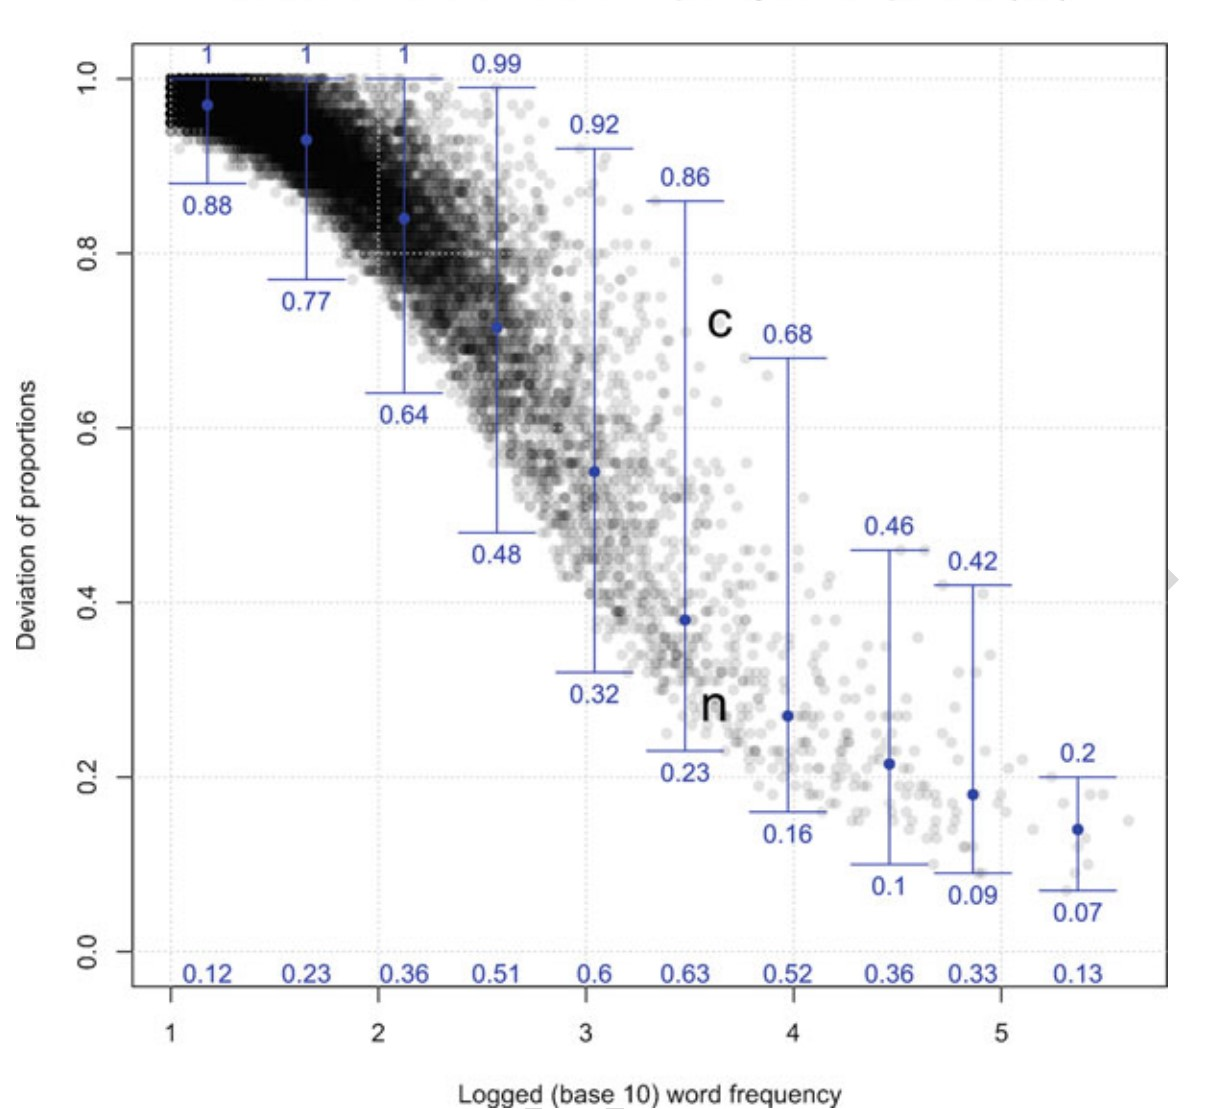
\includegraphics[width=\linewidth]{Gries-frequency-vs-dispersion.jpg}
  \caption[The relation between word frequency and dispersion (DP)]{The relation between word frequency and dispersion ($DP$) \parentext{from \textcite[112]{Gries2021}}}
  \label{fig:Gries-frequency-vs-dispersion}
\end{figure}

Disparities between token frequency and dispersion are especially common for lexical items in the middle frequencies (between 1,000 and 10,000 tokens), as demonstrated in \figref{fig:Gries-frequency-vs-dispersion} from \textcite[112]{Gries2021}. In this plot, word frequency is shown on the x-axis (logged to the base of 10), and dispersion is shown on the y-axis (measured using \dfn{Deviation of Proportions} [$DP$]; see below for details). Each word in the corpus is represented by a gray point. Lexical items are divided into 10 bins based on frequency, and the blue whisker in each bin represents the range of dispersion values in that frequency bin. The plot makes clear just how widely words within the same frequency bin can vary in terms of their dispersion, especially in the middle frequencies.

If what we are intending to capture with these statistics is some idea of the regularity with which speakers encounter a word, it is clear that raw frequency is a deceptive measure. Instead, recent work has shown that \dfn{corpus dispersion}—how evenly an item is distributed in a corpus—more accurately represents frequency of exposure or lexical access \parencites{Gries2008}{Gries2010}{Griesfc}. Corpus dispersion correlates more strongly with reaction time data than does frequency, for example \parencite{Griesfc}.

Thus for this project I report a measure of corpus dispersion in addition to relative token frequency. I use a measure called \dfn{Deviation of Proportions} ($DP$), created by \textcite{Gries2008}. In a review of various measures of corpus dispersion, \textcite{Gries2008} discusses shortcomings with existing measures and proposes Deviation of Proportions as a conceptually simple alternative; it is also this measure which most strongly correlates with reaction time data, as mentioned above. In essence, Deviation of Proportions measures how much the frequency of an item within the various parts of a corpus deviates from what one would expect if the item were evenly distributed in the corpus. The procedure for calculating $DP$ for a given lexical item is as follows:

\begin{enumerate}
  \item Determine the sizes of each part of the corpus as a percentage of the overall corpus. These values represent the \emph{expected} percentage of the time that one would expect the item to appear in each corpus part, if it were evenly distributed.
  \item Determine the frequencies with with the target item occurs in each part, as a percentage of its overall frequency of occurrence. These values represent the \emph{actual} or \emph{observed} percentage of the time that the item apperas in each corpus part.
  \item Compute the pairwise absolute differences between the expected and observed percentages, sum them up, and divide the result by two.
  \item The result is $DP$, which theoretically ranges from $0$ (the item is evenly distributed across the corpus, given the size of the parts) to $1$ (the item is unevenly distributed across the corpus, given the size of the parts).
\end{enumerate}

\noindent The mathematical formulization of $DP$ is shown in \exref{ex:DP}, where $n$ is the number of corpus parts, $v$ is the frequencies of the target item in each corpus part, $f$ is the overall frequency of the target item in the corpus, and $s$ is the percent size of each corpus part.

\begin{exe}
  \ex\label{ex:DP}
  $DP = 0.5 \times \displaystyle\sum_{i = 1}^{n}|\frac{v_i}{f} - s_i|$
\end{exe}

\noindent A more detailed explanation of this calculation, with examples, is in \textcite[§3]{Gries2008}. Note that while the theoretical range of $DP$ is between $0$ and $1$, it will never actually reach these two limits because a particular proportion of the lexical item was expected to occur in each corpus part anyway. This issue is only noticeable in corpora with a very small number of parts.

For this study, each text within the selected corpora is treated as a single corpus part. The spoken portion of the Open American National Corpus contains 2,410 texts, each contained within its own separate file. The Nuuchahnulth corpus contains 24 texts, also each contained within its own file.

Both the token frequencies and corpus dispersions of each lexical item in the 100-item samples are reported in \appref{app:100-item-samples}.

\section{Summary}
\label{sec:3.5}

This chapter has presented the methodological tools necessary for answering the research questions put forth in \chref{ch:introduction}. The methods adopted in this study are novel for several reasons. First, this is the first study to utilize naturalistic discourse data from corpora to examine lexical polyfunctionality at the level of the individual lexical item. Second, this is the first study to \emph{quantify} the lexical polyfunctionality of individual lexical items, in a crosslinguistically applicable way. The calculation of functional diversity using Shannon's $H$ is intended as the main methodological contribution of this dissertation. Finally, this study incorporates findings from recent research in corpus linguistics which suggest that corpus dispersion is a better measure of frequency of exposure than just raw token frequency. As such, I report on both token frequency and corpus dispersion and examine their interaction as they relate to lexical polyfunctionality in \secref*{sec:4.5}. With these methodological prerequisites in place, I now turn to answering this study's research questions in \chref{ch:results}.
